%%**************************************************************
%% Vorlage fuer Bachelorarbeiten (o.ä.) der DHBW
%%
%% Autor: Tobias Dreher, Yves Fischer
%% Datum: 06.07.2011
%%**************************************************************

\newcommand{\pdftitel}{Entwicklung eines Web Based Training Systems nach einem Lernmodell}
\newcommand{\autor}{Michael Gruben \& Julian Babics \& Benjamin Merkle}
\newcommand{\arbeit}{Studienarbeit}

%
% Nahezu alle Einstellungen koennen hier getaetigt werden
%

\documentclass[%
	pdftex,
	oneside,		% Einseitiger Druck.
	12pt,			% Schriftgroesse
	parskip=half,	% Halbe Zeile Abstand zwischen Absätzen.
	headsepline,	% Linie nach Kopfzeile.
	footsepline,	% Linie vor Fusszeile.
	abstracton,	    % Abstract Überschriften
	ngerman,		% Translator
]{scrreprt}

%Seitengroesse
\usepackage{fullpage}

%Zeilenumbruch und mehr
\usepackage[activate]{microtype}

% Zeichencodierung
\usepackage[utf8]{inputenc}
\usepackage[T1]{fontenc}

% Zeilenabstand
\usepackage[onehalfspacing]{setspace}

% Index-Erstellung
\usepackage{makeidx}

% Lokalisierung (neue deutsche Rechtschreibung)
\usepackage[ngerman]{babel}

% Anführungszeichen 
\usepackage[babel,german=quotes]{csquotes}
%\usepackage[style=swiss]{csquotes}


% Spezielle Tabellenform fuer Deckblatt
\usepackage{longtable}
\setlength{\tabcolsep}{10pt} %Abstand zwischen Spalten
\renewcommand{\arraystretch}{1.5} %Zeilenabstand

% Grafiken
\usepackage{graphicx}

% Mathematische Textsaetze
%\usepackage{amsmath}
%\usepackage{amssymb}

% Pakete um Textteile drehen zu können, oder eine Seite Querformat anzeigen kann.
%\usepackage{rotating}
%\usepackage{lscape}

% Farben
\usepackage{color}
\definecolor{LinkColor}{rgb}{0,0,0}
\definecolor{ListingBackground}{rgb}{0.92,0.92,0.92}

% PDF Einstellungen
\usepackage[%
	pdftitle={\pdftitel},
	pdfauthor={\autor},
	pdfsubject={\arbeit},
	pdfcreator={pdflatex, LaTeX with KOMA-Script},
	pdfpagemode=UseOutlines, % Beim Oeffnen Inhaltsverzeichnis anzeigen
	pdfdisplaydoctitle=true, % Dokumenttitel statt Dateiname anzeigen.
	pdflang=de % Sprache des Dokuments.
]{hyperref}

% (Farb-)einstellungen für die Links im PDF
\hypersetup{%
	colorlinks=true, % Aktivieren von farbigen Links im Dokument
	linkcolor=LinkColor, % Farbe festlegen
	citecolor=LinkColor,
	filecolor=LinkColor,
	menucolor=LinkColor,
	urlcolor=LinkColor,
	bookmarksnumbered=true % Überschriftsnummerierung im PDF Inhalt anzeigen.
}

\usepackage{html}
\usepackage[hyphenbreaks,preserveurlmacro]{breakurl}
\usepackage[dcucite]{harvard}
\renewcommand{\harvardand}{und}

% Verschiedene Schriftarten
%\usepackage{goudysans}
%\usepackage{lmodern}
%\usepackage{libertine}
\usepackage{palatino} 

% Hurenkinder und Schusterjungen verhindern
% http://projekte.dante.de/DanteFAQ/Silbentrennung
\clubpenalty=10000
\widowpenalty=10000
\displaywidowpenalty=10000

% Quellcode
\usepackage{listings}
\lstloadlanguages{Java}
\lstset{%
	language=PHP,		 	 % Sprache des Quellcodes
	%numbers=left,           % Zelennummern links
	stepnumber=1,            % Jede Zeile nummerieren.
	numbersep=5pt,           % 5pt Abstand zum Quellcode
	numberstyle=\tiny,       % Zeichengrösse 'tiny' für die Nummern.
	breaklines=true,         % Zeilen umbrechen wenn notwendig.
	breakautoindent=true,    % Nach dem Zeilenumbruch Zeile einrücken.
	postbreak=\space,        % Bei Leerzeichen umbrechen.
	tabsize=2,               % Tabulatorgrösse 2
	basicstyle=\ttfamily\footnotesize, % Nichtproportionale Schrift, klein für den Quellcode
	showspaces=false,        % Leerzeichen nicht anzeigen.
	showstringspaces=false,  % Leerzeichen auch in Strings ('') nicht anzeigen.
	extendedchars=true,      % Alle Zeichen vom Latin1 Zeichensatz anzeigen.
	captionpos=b,            % sets the caption-position to bottom
	backgroundcolor=\color{ListingBackground} % Hintergrundfarbe des Quellcodes setzen.
}

% Glossar
\usepackage[
	nonumberlist, %keine Seitenzahlen anzeigen
	acronym,      %ein Abkürzungsverzeichnis erstellen
	%section,     %im Inhaltsverzeichnis auf section-Ebene erscheinen
	toc,          %Einträge im Inhaltsverzeichnis
]{glossaries}

\usepackage[printonlyused,footnote]{acronym}

%Remove the dot at the end of glossary descriptions
\renewcommand*{\glspostdescription}{}

% Fussnoten
\usepackage[perpage, hang, multiple, stable]{footmisc}

\graphicspath{{images/}}

% Titel, Autor und Datum
\title{\titel}
\author{\autor}
\date{\datum}

\usepackage{bookmark}

\usepackage{float}

\usepackage{array}

\usepackage[right]{eurosym}

\usepackage{wrapfig}

\usepackage{comment}
\specialcomment{k}{\begingroup\color{red}}{\endgroup}
%\excludecomment{k}

\usepackage{pifont} 

% Ab jetzt können auch Umlaute verwendet werden
\newcommand{\titel}{\pdftitel}
\newcommand{\martrikelnr}{2788654}
\newcommand{\kurs}{TAI10B1}
\newcommand{\datumAbgabe}{Mai 2013}
\newcommand{\firma}{M+M, Medical Solutions, SAP AG}
\newcommand{\firmenort}{Pforzheim, Karlsruhe, Roth}
\newcommand{\abgabeort}{Karlsruhe}
\newcommand{\abschluss}{Bachelor of Science}
\newcommand{\studiengang}{Studienganges Angewandte Informatik}
\newcommand{\dhbw}{Karlsruhe}
\newcommand{\betreuer}{Dr. Kay Margareth Berkling}
\newcommand{\gutachter}{Prof. Dr. Johannes Freudenmann}
\newcommand{\zeitraum}{2,5 Monate}
\newcommand{\arbeitsart}{\arbeit}

\makeglossaries
%
% vorher in Konsole folgendes aufrufen: 
%	makeglossaries makeglossaries dokumentation.acn && makeglossaries dokumentation.glo
%

%
% Abkürzungen --> referenz, name, beschreibung
% Aufruf mit \gls{...} oder Kurzform mit \acrshort{...}
%

\newacronym{DHBW}{DHBW}{Duale Hochschule Baden Württemberg}
\newacronym{I2CBus}{I\textsuperscript{2}C-Bus}{Inter-Integrated-Circuit-Bus}

%
% Glossareintraege --> referenz, name, beschreibung
% Aufruf mit \gls{...}
%
\newglossaryentry{Glossareintrag}{name={Glossareintrag},plural={Glossareinträge},description={Ein Glossar beschreibt verschiedenste Dinge in kurzen Worten}}


\begin{document}

	% Deckblatt
	\begin{spacing}{1}
		\begin{titlepage}
	\begin{longtable}{p{.55\textwidth} p{.85\textwidth}}
	  {} & 
	  {
\includegraphics[height=2.6cm]{dhbw.png}}
	\end{longtable}
	\enlargethispage{20mm}
	\begin{center}
	  \vspace*{12mm}	{\LARGE\bf \titel }\\
	  \vspace*{12mm}	{\large\bf \arbeit}\\
	  \vspace*{12mm}	für die Prüfung zum\\
	  \vspace*{3mm} 	{\bf \abschluss}\\
	  \vspace*{12mm}	des \studiengang\\
	  \vspace*{3mm} 	an der Dualen Hochschule Baden-Württemberg \dhbw\\
	  \vspace*{12mm}	von\\
	  \vspace*{3mm} 	{\large\bf Michael Gruben \normalsize\rm Meyle+Müller
	  GmbH+Co.KG (Pforzheim) \phantom{iiiiibH (Bruchsal)     }\&}\\
	  \vspace*{3mm} 	{\large\bf Julian Babics \normalsize\rm MedicalCommunications
	  Soft- und Hardware GmbH (Bruchsal) \&}\\
	  \vspace*{3mm} 	{\large\bf Benjamin Merkle \normalsize\rm SAP AG (Walldorf)
	  \phantom{mniiiiiiiiiiiiiiiiiiiiiiiiiiiiiiiiiiiiibH (Bruchsal)}}\\
	  \vspace*{12mm}	\datumAbgabe\\
	\end{center}
	\vfill
	\begin{spacing}{1.2}
	\begin{tabbing}
		mmmmmmmmmmmmmmmmmmmmmmmmmm     \= \kill
		\textbf{Bearbeitungszeitraum}  \>  \zeitraum\\
		\textbf{Matrikelnummer, Kurs}  \>  \martrikelnr, \kurs\\
		%\textbf{Ausbildungsfirmen}      \>  Meyle+Müller GmbH+Co.KG (Pforzheim)\\
		%\>MedicalCommunications Soft- und Hardware GmbH (Bruchsal)\\
		%\>SAP Deutschland AG & Co. KG (Walldorf)\\
		\textbf{Betreuer}              \>  \betreuer\\
 		\textbf{Gutachter}             \>  \gutachter
	\end{tabbing}
	\end{spacing}
\end{titlepage}
	\end{spacing}
	\newpage

\renewcommand{\thepage}{\Roman{page}}
	\setcounter{page}{1}
	
	% Sperrvermerk
% 	\thispagestyle{empty}
% Sperrvermerk direkt hinter Titelseite
\section*{Sperrvermerk}

\vspace*{2em}

Die vorliegende {\arbeitsart} mit dem Titel {\itshape \titel} ist mit einem Sperrvermerk versehen und wird ausschließlich zu Prüfungszwecken am Studiengang {\studiengang} der Dualen Hochschule Baden-Württemberg {\abgabeort} vorgelegt.
Jede Einsichtnahme und Veröffentlichung – auch von Teilen der Arbeit – bedarf der vorherigen Zustimmung durch die {\firma}.
% 	\newpage
	
	% Erklärung
	\thispagestyle{empty}

\section*{Erklärung}
% http://www.se.dhbw-mannheim.de/fileadmin/ms/wi/dl_swm/dhbw-ma-wi-organisation-bewertung-bachelorarbeit-v2-00.pdf
\vspace*{2em}

Ich erkläre hiermit ehrenwörtlich: \\
\begin{enumerate}
\item dass ich meine {\arbeitsart} mit dem Thema
{\itshape \titel } ohne fremde Hilfe angefertigt habe;
\item dass ich die Übernahme wörtlicher Zitate aus der Literatur sowie die Verwendung der Gedanken
anderer Autoren an den entsprechenden Stellen innerhalb der Arbeit gekennzeichnet habe;
\item dass ich meine {\arbeitsart} bei keiner anderen Prüfung vorgelegt habe;
\item dass die eingereichte elektronische Fassung exakt mit der eingereichten schriftlichen Fassung
übereinstimmt.
\end{enumerate}

Ich bin mir bewusst, dass eine falsche Erklärung rechtliche Folgen haben wird.

\vspace{3em}

\abgabeort, \datumAbgabe
\vspace{4em}

\autor
	\newpage

	% Abstract
	\pagestyle{empty}

\renewcommand{\abstractname}{Zusammenfassung}

\begin{abstract}
Im Verlauf der Bearbeitung der Studienarbeit "`Analyse und Vergleich von
Autorensystemen für ein WBT zu Vorlesungsinhalten"' ist in der Vorlesung
"`Gamification"' ein Konzept für ein WBT\footnote{Web Based Training}-System
entstanden. Aus dieser Vorstellung ist die Idee, und damit die Motivation der
Studienarbeit, entstanden es in die Realität umzusetzen.

Es handelt sich um eine Webapplikation, die diverse WBTs in entsprechenden
Kategorien zum Bearbeiten anbietet. Das Lernmodell der Gebrüder Dreyfuß
wird in diese verwoben. In dem Modell wird die Kompetenz in einem Fachgebiet auf
zwei unterschiedlichen Ebenen betrachtet, die fachliche Kompetenz und die
Fähigkeit erklären zu können.

Zunächst wird die fachliche Kompetenz betrachtet. Demnach bearbeitet ein Neuling
auf dem ersten Kompetenzlevel eines bestimmten Fachbereiches ein grundlegendes
WBT, dessen abschließende Fragen nach vorgegebenen Schemata und grundlegender
Eigenschaften beantwortet werden. Ein Experte auf dem vierten Kompetenzlevel
muss hingegen Antworten auf Fragen wissen, die ein wesentlich komplexeres
Verständnis eines Sachverhaltes verlangen.

Um seine Fähigkeit erklären zu können unter Beweis zu stellen, engagiert man
sich mit Hilfestellungen für niedere fachliche Level. Beurteilen diese die
Hilfestellung als gut, kann der Mastery Rang erreicht werden, der sich noch über
dem Experten befindet. Nach dem Dreyfuß-Modell dürfen sich Lernender und
Lehrender durch maximal zwei Level unterscheiden. Der Mastery-Level ist hingegen
ein "`erklärender Experte"', der nicht nur fachlich höchst Kompetent ist,
sondern auch sehr gut auch für einen Anfänger erklären kann, ohne in fachliche
Details abzuschweifen.

Das WBT-System, welches beide beschriebenen Ebenen der Kompetenz organisiert,
wird unter einer freien Lizenz veröffentlicht werden. So kann das als noch sehr
simpel und eingeschränkt erwartete Ergebnis der Studienarbeit als Community
Projekt weiterleben und weiterentwickelt werden. Bereits vor Bearbeiten der
Studienarbeit wird damit gerechnet, das nur ein kleiner und spezieller aber
funktionaler Teil des Konzeptes umgesetzt werden wird. Der Fokus liegt
dabei grundsätzlich mehr auf Funktionalität, einer leicht zu erweiternden
Architektur der Software und einem benutzerfreundlichem Interface, als auf
einem gut aussehendem Design.
\end{abstract}
% \begin{abstract}
% Ein Abstract ist eine prägnante Inhaltsangabe, ein Abriss ohne
% Interpretation und Wertung einer wissenschaftlichen Arbeit. In DIN
% 1426 wird das (oder auch der) Abstract als Kurzreferat zur
% Inhaltsangabe beschrieben.
% 
% \begin{description}
% \item[Objektivität] soll sich jeder persönlichen Wertung enthalten
% \item[Kürze] soll so kurz wie möglich sein
% \item[Genauigkeit] soll genau die Inhalte und die Meinung der Originalarbeit wiedergeben
% \end{description}
% 
% Üblicherweise müssen wissenschaftliche Artikel einen Abstract
% enthalten, typischerweise von 100-150 Wörtern, ohne Bilder und
% Literaturzitate und in einem Absatz.
% 
% Quelle \url{http://de.wikipedia.org/wiki/Abstract} Abgerufen 07.07.2011
% \end{abstract}
% 
% 
% \renewcommand{\abstractname}{Summary}
% \begin{abstract}
% An abstract is a brief summary of a research article, thesis, review,
% conference proceeding or any in-depth analysis of a particular subject
% or discipline, and is often used to help the reader quickly ascertain
% the paper's purpose. When used, an abstract always appears at the
% beginning of a manuscript, acting as the point-of-entry for any given
% scientific paper or patent application. Abstracting and indexing
% services for various academic disciplines are aimed at compiling a
% body of literature for that particular subject.
% 
% The terms précis or synopsis are used in some publications to refer to
% the same thing that other publications might call an "abstract". In
% management reports, an executive summary usually contains more
% information (and often more sensitive information) than the abstract
% does.
% 
% Quelle: \url{http://en.wikipedia.org/wiki/Abstract_(summary)}

% \end{abstract}

\newpage
\thispagestyle{empty}
\vspace*{\fill}
\begin{quotation}
\textit{"`Die meisten Menschen sind bereit zu lernen, aber nur die wenigsten, sich belehren zu lassen."'}\\
{\footnotesize Winston Churchill, Britischer Politiker und Nobelpreisträger,
1874 - 1965.}
\end{quotation}
\vfill
	\newpage

	\pagestyle{plain}

	% Inhaltsverzeichnis
	\begin{spacing}{1.1}
		\setcounter{tocdepth}{2}
		\tableofcontents
	\end{spacing}
	\newpage

	\setglossarysection{chapter}
	% Abkürzungsverzeichnis
	% vorher in Konsole folgendes aufrufen: 
	%	makeglossaries makeglossaries dokumentation.acn && makeglossaries dokumentation.glo
	%\printglossary[type=\acronymtype,title=Abkürzungsverzeichnis,toctitle=Abkürzungsverzeichnis]
	\cleardoublepage
	\phantomsection \label{listofacs}
	\addcontentsline{toc}{chapter}{Abkürzungsverzeichnis}
	\chapter*{Abkürzungsverzeichnis}

\begin{acronym}[WYSIWYG]
\newcommand{\acrov}{\vspace{\parsep}}
\setlength{\itemsep}{-\parsep}
\acro{ADL}{Advanced Distributed Learning}
\acro{AGPL}{Affero GNU General Public License}
\acro{API}{Application Programming Interface}
\acrov
\acro{CAM}{Content Aggregation Model}
\acro{CBT}{Computer Based Training}
\acrov
\acro{DE}{Distance Education}
\acro{DRY}{Don't repeat yourself}
\acrov
\acro{F2F}{Face-To-Face}
\acrov
\acro{GPL}{GNU General Public License}
\acro{GUI}{Graphical User Interface}
\acrov
\acro{HTML}{Hypertext Markup Language}
\acrov
\acro{KISS}{Keep it simple stupid'}
\acrov
\acro{LMS}{Learning Management System}
\acrov
\acro{MVC}{Model View Control}
\acrov
\acro{OE}{Online Education}
\acrov
\acro{PIF}{Package Interchange File}
\acrov
\acro{RoR}{Ruby on Rails}
\acro{RTE}{Run Time Environment}
\acrov
\acro{SCO}{Shared Content Object}
\acro{SCORM}{Shared Content Object Reference Model}
\acrov
\acro{WBT}{Web Based Training}
\acro{WYSIWYG}{What You See Is What You Get}
\acrov
\acro{YAGNI}{You ain't gonna need it}
\end{acronym}

	% Glossar
	\printglossary[style=altlist,title=Glossar]
	
	\newpage
		
	\renewcommand{\thepage}{\arabic{page}}
	\setcounter{page}{1}
	
	% Inhalt
	\chapter{Einleitung}\label{ref:chaptIntroduction}
Basierend auf der Studienarbeit "`Analyse von Authorensystemen für ein WBT zu
Vorlesungszwecken von Michael Gruben \cite{gruben:2012} wird in dieser
Studienarbeit ein System aus \ac{WBT}s geschaffen. Das Konzept für das
Produkt des Projektes ist im Rahmen der Vorlesung "`Gamification"' entstanden.

Dabei handelt es sich grundsätzlich um eine Blended Learning Plattform, die
interessierten Lernenden eine zentrale Anlaufstelle bietet. Es werden also
eLearning und persönliches Lernen miteinander kombiniert. Umrahmt und
gamifiziert wird die Idee mithilfe des Dreyfus fünf Etappen Modells mentaler
Aktivitäten. Die in dieser Studienarbeit verwendeten Bezeichnungen unterliegen
gegebenenfalls weiteren Änderungen und sind für die deutschsprachige Version der
Plattform bestimmt.

Inhalte der vorligenden Studienarbeit sind Einblicke in die Entwicklung des
ersten Prototyps. Dazu zeigt Kapitel \ref{ref:chaptConcept} die Konzeption und
damit die grundlegende Idee der Architektur. Daran anschließend wird in Kapitel
\ref{ref:chaptScript} näher auf den tatsächlichen Entwurf eingegangen. Hier
wird konkret auf Klassen und Methoden eingegangen, welche die Realisierung
bestimmter Use-Cases zum Ziel haben. Kapitel \ref{ref:chaptImplementation}
zeigt, wie der Entwurf letztlich realisiert wird. Hier sind auch erste
Screenshots der Anwendung zu sehen. Um die vorrangegangenen Schritte
zusammenzufassen und kurz auszuwerten, gibt Kapitel \ref{ref:chaptConclusion}
einen Gesamtüberblick. Darauf aufbauend bietet Kapitel \ref{ref:chaptSummary}
eine Auswertung, die alle Aspekte des Projekts umfasst. Zusätzlich werden hier
Ausblicke auf die weitere Verwendung des Projektergebnisses gegeben.

Am Ende des Projekts steht ein funktionierender Prototyp, der die wesentlichen
Funktionen beherrscht. Weiterhin wird ein Konzept entwickelt worden sein,
welches das Projekt an zentralen Stellen bekannt macht und so für eine rege
Beteiligung sorgen soll. Mit der Namensgebung "`Masterly Mate"'\footnote{weitere
Details zur Namensgebung in Abschnitt \ref{ref:naming}} wurde bereits vor dem
eigentlichen Projektstart ein wesentlicher Schritt zur Bekanntmachung getan.
	\part{Vorbereitungen}
	\chapter{Projektplanung}
Die Projektidee entstammt von studentischer Seite. In Abbildung
\ref{ref:wolkeMM} ist eine Wortwolke zu sehen, in der in Stichworten beschrieben
ist, was sich unter Masterly Mate vorzustellen ist.

\begin{figure}[H]
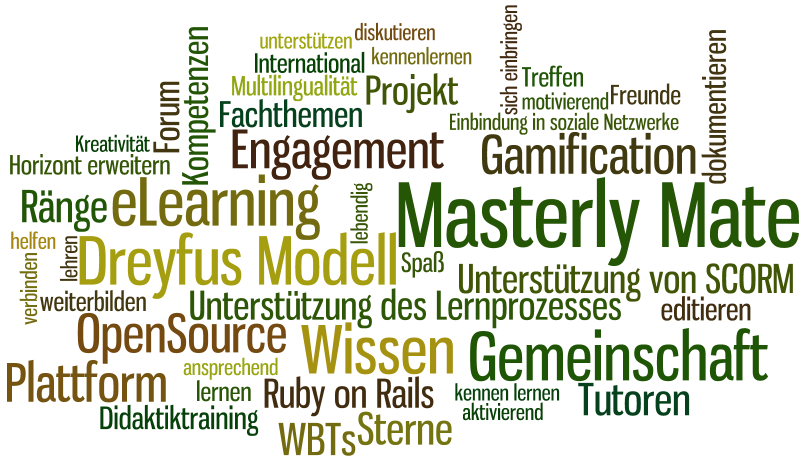
\includegraphics[width=1\textwidth]{MasterlyMateWolke.png}
\caption{Wortwolke über die "`Masterly Mate"'-Idee}\label{ref:wolkeMM}
\end{figure}

Das Projekt nimmt sich eine Art Lernplattform zum Ziel, auf der Lernende auf
Lehrende treffen sollen. Dabei entstehen Situationen, in der eine lehrende
Person zu einer lernenden wird, und umgekehrt. Es sollen Diskussionen über
bestimmte Fachgebiete stattfinden können und ideale Tutoren für bestimmte
Fragestellungen gefunden werden. Da es nichts zu gewinnen gibt, engagiert sich
jeder Teilnehmer freiwillig. Er erhält Wissen und kann dieses im nächsten Moment
an weitere interessierte Personen weitergeben, was sein eigenes Wissen erneut
festigt. Lehrstunden sollen im gemütlichen Umfeld, wie Caffees oder Parks
stattfinden. Masterly Mate bietet dazu eine regionale Suche an, mit deren Hilfe
Lernende und Lehrende aufeinander treffen. Dem Duo steht es auch offen auf
andere Kommunikationskanäle, wie Chat oder E-Mail, zu wechseln. Jeder Nutzer
kann als Tutor für sein Fachgebiet oder seine Fachgebiete fungieren.

Um stets einen idealen Tutor zu finden, folgt die Idee dem Dreyfus fünf Etappen
Modell mentaler Aktivitäten, welches in Abschnitt \ref{ref:dreyfus} näher
beschrieben wird. So ist gewährleistet, dass ein Neuling die Inhalte von einer
Person erklärt bekommt, die selbst noch im Lernprozess steckt und es können
Inhalte, Tipps und Hinweise auf passendem Niveau ausgetauscht werden.

Letztlich soll das Ziel der Mitgliedschaft auf der Plattform nicht sein, der
beste Guru eines Faches zu werden oder der beste Lehrer zu werden. Es geht darum
Teil einer Bildungsgemeinschaft zu sein und sich gegenseitig engagiert zu
unterstützen.

\section{Motivation und Notwendigkeit}\label{ref:projectMotivation}
Die Motivation zu dieser Idee entstand aus der interessanten und
erwartungsvollen Kombination von eLearning und Gamification. Hinzu kommt die
heute populäre Vorstellung von Blended Learning, wodurch das doch sehr trockene
und eintönige Durcharbeiten von WBTs durch Lehreinheiten mit einem Tutor
unterstützt wird.

Masterly Mate soll eine zentrale Anlaufstelle für diverse Weiterbildungs- und
Lernangelegenheiten sein. Unabhängig davon, ob die Motivation privatem Interesse
oder dem eigenen Bildungsweg entspringt, soll jeder Interessent wissen, dass
die Plattform Antworten bietet.

Die Notwendigkeit resultiert aus der fehlenden Fähigkeit des Internets,
Sachverhalte erläutern zu können. Heute ist es Usus beim Recherchieren das
Internet zu gebrauchen, in dem rohe Daten und Informationen vorliegen. Wissen
ist dort eher rar. Es gibt bisher nur wenige Plattformen, wie Wikipedia, die
existieren, um Wissen zu publizieren, jedoch fehlt auch dort eine erklärende und
erläuternde Komponente durch einen Menschen. Dieses Manko soll Masterly Mate
ausgleichen.

\section{Abgrenzung}
Das Projektergebnis behauptet keinen Anspruch auf ein vollwertiges \ac{LMS}. Es
fehlt die Komponente zur Organisation kompletter Lernpakete. In Masterly Mate
stehen die WBTs unabhängig da. Sie sind allein Mittel zum Zweck als Beleg für
die fachliche Kompetenz.

Weiterhin soll es Wikipedia nicht ersetzen. Das Projektergebnis bietet keine
ausformulierten Texte oder Artikel zu Lerninhalten. Der Fokus liegt wesentlich
stärker auf der Komponente Wissen zu vermitteln.

\section{Zielsetzung}
Da das Projekt insgesamt auf einen längeren Zeitraum angesetzt ist, lässt es
sich nicht innerhalb der Bearbeitungszeit der vorliegenden Studienarbeit
umsetzen. Aus diesem Grund sind die Ziele zum einen in operative und zum anderen
in strategische zu unterteilen. 

\subsection{Operative Ziele}
Wie in Kapitel \ref{ref:chaptIntroduction} bereits angerissen wurde, soll zu
Projektende ein funktionaler Prototyp stehen. Auch ist ein Konzept angedacht,
welches der Bekanntmachung von Masterly Mate dient. Eventuell wird sich bis
dahin eine kleine, lebendige Gemeinschaft gebildet haben, die die Plattform
nutzt und um Inhalte erweitert. Die ersten Nutzer sollen automatisch unabhängig
ihres didaktischen Grades\footnote{näher erläutert in Abschnitt
\ref{ref:rankTeach}} Autoren sein. So ist gewährleistet, dass Inhalte für neue
Nutzer bereits existieren. 

Das Projekt als Ganzes soll einen leichten Start haben. Sind die Ziele für die
ersten Nutzer zu hoch gesteckt, resultiert aus der geringen Anzahl von Nutzern
und der damit schwer erreichbaren nächsten Rängen Frustration und Unwille zur
Nutzung der Plattform. Somit ist angedacht, die erforderliche Punktzahl für
höhere Ränge (siehe Abschinitt \ref{ref:dreyfus}) mit der Menge der Nutzer zu
skalieren.

\subsection{Strategische Ziele}
Längerfristig betrachtet soll eine rege und große Gemeinschaft entstehen, die
Hilfsbereitschaft nicht scheut. Dazu wird bereits zu Beginn der Entwicklung eine
Internationalisierung\footnote{siehe Abschnitt \ref{ref:internationalisierung}}
berücksichtigt. Masterly Mate soll zur, in Abschnitt \ref{ref:projectMotivation}
beschriebenen, zentralen Anlaufstelle heranwachsen.

Dabei werden, um den Reiz am Lernen zu erhöhen, mit der Menge der Nutzer die
Anforderungen für die jeweils nächsten Ränge erhöht. Denn je mehr Beteiligung
die Plattform erfährt, desto wahrscheinlicher ist es, einen Tutor in der
jeweiligen Region zu finden. Damit wird es auch immer einfacher, Punkte für den
didaktischen Rang zu sammeln.
	\chapter{Theoretische Grundlagen}
Das Projekt basiert auf einigen theoretische Grundlagen. Dazu zählen
Lerntheorien und technische Begriffe, deren Erläuterungen Inhalt
dieses Kapitels sind. Dabei handelt es sich um eine Kurzfassung der
Beschreibungen aus \cite{gruben:2012}.

\section{Lernen}
Das Lernen selbst wird heute als ein Prozess verstanden. Dabei wirken "`mehrere
zentrale psychologische Phänomene (Motivation, Emotion,
Kognition)"'\cite{niegemann:2004} zusammen. 

Der Lernprozess besteht dabei aus drei Abschnitten:
\begin{enumerate}
  \item Zunächst werden Eindrücke wahrgenommen. Dabei tragen neue oder
  vergessene Eindrücke zur Umstrukturierung im Gehirn bei.
  \item Umstrukturieren bedeutet, dass Synapsen bewegt und andere Gehirnzellen
  angekoppelt werden.
  \item Mit Wiederholungen wird Wissen persistiert. Es entstehen stabile
  Strukturen, welche einfach und schnell abrufbar sind.
\end{enumerate}
In Abbildung \ref{pic:structSyn} wird diese Umstrukturierung illustriert
\cite{spitzer:2012}.

Von ein LMS wird erwartet, dass es diesen Lernprozess unterstützt. Anfänger
sollen die Möglichkeit erhalten zunächst klein anzufangen und die Grundlagen
eines bestimmten Sachverhaltes kennenzulernen. Fortschreitend können die
Anforderungen und Herausforderungen gesteigert werden, um den Lernprozess zu
unterstützten und zugleich die Motivation aufrecht zu erhalten.

\begin{figure}[H]
\centering
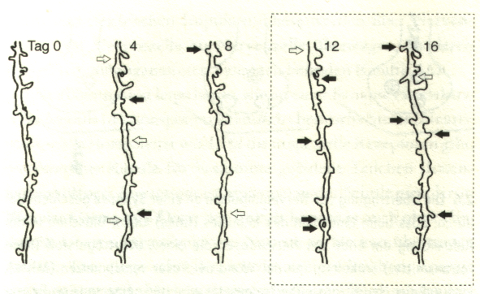
\includegraphics[width=0.7\textwidth]{SPIsynapseS50.png}
\caption{Umstrukturierung von Synapsen \footnotemark}\label{pic:structSyn}
\end{figure}\footnotetext{aus \cite{spitzer:2012}}

\section{Motivation}
Die Motivation ist ein wesentliches Standbein des Lernprozesses. Fehlt sie, so
ist es für Lernende bedeutend erschwert, Lerninhalte aufzunehmen, zu verarbeiten
und zu verstehen. Mithilfe von Motivation wird ein charakteristisches Verhalten
an den Tag gelegt, welches den Lernprozess aufrecht erhält \cite{jacobs:2010}.

Im Mittelpunkt jeder Motivation steht stets das persönliche Glück
\cite{stampfl:2012}. Dabei stehen Mittel zur Verfügung, die dem Lernenden auf
unterschliedliche weise unterstützen zu verstehen. Er kann zum einen
intrinsisch und zum anderen extrinsisch motiviert werden.

\subsection{Intrinsische Motivation}\label{ref:intrinsischeMotivation}
Die intrinsische Motivation wird auch als direkte Motivation bezeichnet. Damit
wird der Lernende direkt angesprochen und in seinen Bedürfnissen befriedigt und
seinen Wünschen wird unmittelbar nachgegangen. Ein intrinsisch motivierter
Lernender geht einer Tätigkeit im eigenen Interesse nach, es sind keine externen
Einflüsse nötig, die ihn zu seinen Handlungen erst bewegen müssen
\cite{jacobs:2010}.

Jede Lernsoftware hat aus dem zuvor erwähnten Sachverhalt die intrinsiche
Motivation zum Ziel. Dazu werden nicht selten unter Anderem auch gamifizierende
Inhalte verwendet (siehe \ref{ref:gamification}).

\subsection{Extrinsische Motivation}
Die andere Seite der Motivation kommt von aussen. Es werden Belohnungen gegeben
oder Strafe und negative Konsequenzen vermieden. Synonyme sind demnach
"`indirekte Motivation"', das "`Butterbrot-und-Peitsche-Prinzip"' oder
"`Manipulation"' \cite{jacobs:2010}.

Für Masterly Mate im Speziellen, kann der Tutor ein extrinsisch Motivierender
Faktor sein. Hinzu kommen die gamifizierenden Elemente der zu erreichenden
Punktzahl pro WBT und das Aufsteigen in Rängen. Implizit wird auch Strafe in der
Form angewandt, dass es laut Konzept auch möglich ist, im Rang zu fallen
(siehe dazu Tabelle \ref{tab:privilegesRoles}).

\section{Lernmodelle}
Zum Zweck der Unterstützung des Lernprozesses und Förderung der Motivation haben
sich einige Lernmodelle herauskristallisiert, die heute als gültig und
vertretbar angesehen werden. In der Idee von MasterlyMate sind explizit zwei
Lernmodelle verwoben. Das Dreyfus fünf Etappen Modell mentaler Aktivitäten und
Blended Learning.

\subsection{Das Dreyfus fünf Etappen Modell mentaler
Aktivitäten}\label{ref:dreyfus}
Inhalt des Dreyfus-Modells ist das Hinterfragen, welche Person einer anderen
einen bestimmten Sachverhalt erklären sollte. Dabei wird insbesondere
berücksichtigt, wie groß der Unterschied der Fachkompetenz zwischen Lernenden
und Lehrenden ist. Es wurden insgesamt fünf Ränge\footnote{Novice, Competence,
Proficiency, Expertise, Mastery} definiert, die den Lernweg von abstrakten
Prinzipien hin zu konkreter Erfahrung mit der Aneignung von Wissen beschreiben
\cite{dreyfus:1980}.

Allgemein formuliert sollte kein Experte einem Neuling etwas erklären. Steigt
man neu in ein Fachgebiet ein, so sind zunächst simple und einfache Beispiele
verbunden mit einem engen Betrachtungswinkel des Sachverhalts sehr hilfreich.
Ein Experte würde den Neuling mit unnötigen Details überhäufen.

Dazu staffelt sich der Lernerfolg in fünf Etappen:
\begin{description}
  \item[1. Novize] Ein Novize ist auf grundlegende Anweisungen angewiesen. Er
  verfügt über kein Vorwissen und evaluiert sich nicht selbst. Mit extrinsischem
  Feedback wird dem Abkommen vom Regelwerk zuvorgekommen.
  \item[2. Fortgeschrittener] Die Handlungen des Fortgeschrittene sind gegenüber
  dem Novizen weniger kontextfrei. Sein weiterer Lernweg kann auf seiner kleinen
  Wissensbasis aufbauen. Er hat grundlegende Prinzipien verstanden und erkennt
  situationsbasierte Muster. Der Fortgeschrittene kann simple Beispiele anhand
  von Guidelines durchlaufen, er experimentiert jedoch nicht.
  \item[3. Erfahrener] Der Umgang mit typischen Situationen am ihm gegebenen
  System stellen keine Hürden für den Erfahrenen dar. Ihm ist es möglich neue
  Situationen anzuknüpfen, einzuordnen und sehr ähnliche bewusst zu
  unterscheiden. Der Erfahrene arbeitet nach selbst erschaffenen Maximen.
  \item[4. Experte] Der Experte ist kein geeigneter Lehrer für einen Novizen
  mehr. Er hat die grundlegenden Prinzipien verloren und arbeitet nach seiner
  Intuition, einer Mischung aus Regeln, Guidelines und Maximen. Lösungen für
  ungewohnte Situationen gehören stets zum Reportoir des Experten. Im Sinne der
  fachlichen Kompetenz ist dieser Grad der höchste.
  \item[5. Meister] Ein Meister zeichnet sich gegenüber dem Experten neben
  fachlicher Kompetenz durch herausragende didaktische Fähigkeiten aus. Er
  bleibt damit auch ein geeigneter Lehrer für Novizen.
\end{description}

Generell sollte sich ein Lehrer zwei Grade über seinem Schüler befinden oder
Meister sein. Weitere detailliertere Erklärungen zu den Rängen finden sich in
\cite{gruben:2012}.

\subsection{Blended Learning}\label{ref:blendedLearning}
Zweck des Blended Learning, zu deutsch auch Integriertes Lernen genannt, ist das
Verschmelzen der Vorteile diverser Lernformen. Darunter befinden sich
\ac{F2F}-Education, \ac{DE} und \ac{OE} (eLearning). Die jeweiligen Nachteile
wurden dabei weitestgehend überwunden \cite{kroeger:2004}.

MasterlyMate verfolgt die Verschmelzung von F2F-Education, der Durchführung von
Präsenzunterricht, mit eLearing, dem Durcharbeiten von WBTs. Die DE wird dabei
nur am Rande betrachtet, da nur in Ausnahmefällen Unterweisungen über Chats oder
ähnliche Kommunikationskanäle vonstatten gehen sollen.

\section{eLearning}
Mit dem eLearning wird im Gegensatz zum regulären Lernprozess ein zusätzlicher
Mittler, eine elektronische Komponente, zwischen die rohen Informationen und dem
lernenden Individuum eingeschoben. Heute ist beispielsweise ein Webbrowser ein
Wiedergabemedium von Vielen, welches der Demonstration von Informationen dient
\cite{baumgartner:2002}.

\subsection{Vorteile}
ELearing ist grundsätzlich unabhänig von physischen Gegebenheiten, mithilfe von
Software lassen sich sämtliche, auch fiktive, Szenarien darstellen. Der
Kreativität sind keine Grenzen gesetzt. Auch ist eine enorm vereinfachte
Auswertung von Prüfungen und Tests möglich, da Computer zur Automatisierung von
Prozessen geschaffen sind. 

Für MasterlyMate bedeutet das, dass das Aufsteigen in höhere Ränge automatisiert
vonstatten gehen kann. Beim Überschreiten bestimmter Schwellwerte für Punkte
steigt der Lernende wie von selbst einen Rang auf. Es wird zudem möglich,
Statistiken für den Nutzer anzufertigen, was das Prinzip des gamifizierens
(siehe Abschnitt \ref{ref:gamification}) zusätzlich unterstützt. Das
MasterlyMate selbst ein digitales Produkt ist, spielt darüber hinaus der eigenen
vereinfachten Verbreitung über nationale Grenzen hinweg stark zu.

\subsection{Nachteile}  
Grundsätzlich ist der Unterschied zwischen Mensch und Maschine der größte
Gegner von eLearning. Ein Computer kann heute nur recht spärlich auf die
Bedürfnisse des Lernenden eingehen. 

Expertensystemen wird beispielsweise nur eine beratende Funktion zugeteilt.
Weitere Beispiele sind neuronale Netze, welche zwar Lösungen entwickeln können,
jedoch muss deren Erarbeitung überwacht und hinterfragt werden
\cite{keller:2000}.

Letztlich kann das Lernen am Computer heute nicht die Qualität bieten, die ein
Lernender mit einer Lehrkraft erfährt. Seit 1989 entstehen die selben
Diskussionen um den Einsatz von eLearning in Schulen \cite{thome:1989}.

Im Konzept für MasterlyMate werden diese Nachteile berücksichtigt. Wie in
Abschnitt \ref{ref:blendedLearning} beschrieben, baut der Ansatz nicht allein
auf eLearning. Die Nachteile sind erkannt und werden soweit möglich durch die
Verbindung mit Präsenzveranstaltungen gemildert.

\section{Gamification}\label{ref:gamification}
Ganz nach dem Claim "`Fun is just another word for learning"'\cite{koster:2005},
werden heute mithilfe von Gamification seriöse Inhalte mit spielerischen
Elementen versehen. Damit sollen diese dank geförderter intrinsischer
Motivation (siehe Abschnitt \ref{ref:intrinsischeMotivation}) einfacher zu
vermitteln sein.

MasterlyMate macht sich diese Eigenschaft zunutze. Es werden Fortschrittsbalken
und Statistiken integriert. Zusätzlich erhält er mit höheren fachlichen Level
mehr Möglichkeiten zur Gestaltung seines Profils oder als Tutor für
Gleichgesinnte. Wie die Idee des Gamification in MasterlyMate konkret
konzeptioniert wird, ist Inhalt von Abschnitt \ref{ref:gamificationConcept}.

\begin{k}
hier noch weitere Inhalte und Referenzen aus der Vorlesung Gamification?
\end{k}

\section{Learning Management System}
Ein LMS unterstützt das selbstgesteuerte Lernen. Ein Nutzer arbeitet sich,
möglichst intrinsisch motiviert, durch die ihm dort gebotenen Inhalte
\cite{wendt:2003}.

Wie in der Einleitung beschrieben ist MasterlyMate selbst ein LMS. Der Lernende
entscheidet sich selbst für ein Themengebiet (Topic), welches ihn interessiert.
Dazu findet er WBTs, die ihm bestimmte Sachverhalte auf seinem fachlichen Niveau
näher bringen. MasterlyMate geht mit der Vermittlung von Tutoren über die
eigentliche Definition des LMS hinaus, was es von existierenden OpenSource-LMS,
wie Moodle abgrenzt.

\section{Autorenwerkzeug}
MasterlyMate erfordert das Einbinden von WBTs. Autorenwerkzeuge als
\ac{WYSIWYG}-Editoren dienen deren Erstellung und machen laut Definition das
Einbringen von Multimedia möglich \cite{niegemann:2004}. 

In vielen LMS sind heute simple Autorenwerkzeuge integriert. Externe Lösungen
hingegen lassen sich je nach ihren Möglichkeiten und der Handhabung in
professionelle Autorensysteme, WYSIWYG-Editoren und Rapid Content Development
klassifizieren \cite{niegemann:2004}. MasterlyMate unterstützt mit der
Einbindung von SCORM (siehe Abschnitt \ref{ref:scorm}) alle Varianten und bietet
demgegenüber kein eigenes Werkzeug zum Erstellen von Inhalten an.

\section{WBT}
Beim Begriff des WBTs handelt es sich um eine Softare, die Web-Technologien
nutzt, um eLearning zu realisieren. Blickt man tiefer in die Definition, so
gehen die Meinungen heute auseinander. Eine Variante ist eine Erklärung von
Peter Baumgartner: "`WBT umfasst die internetgestützte Form des Fernlernens mit
und ohne Betreuung durch Tutoren"'\cite{baumgartner:2002}. Dem hinzuzufügen ist,
dass Web-Applikationen im Allgemeinen auch ohne eine Anbindung an das Internet,
beispielsweise lokal oder in einem kleinen Firmennetzwerk, brauchbar sind. 

In einer weiteren Definition taucht das WBT in einer Klassifikation zwischen
virtuellem Klassenzimmer und \ac{CBT} auf. Es kann damit auf eine tutorielle
Betreuung verzichten und ist stark an die Verfügbarkeit in einem
Computernetzwerk gebunden \cite{schleifer:2003}.

Historisch ist WBT aus \ac{DE}, "`Computer-conveyed education"' und diversen
Internet Technologien entstanden, deren Technologien, Traditionen und Techniken
den Grundstein bilden. Daraus wurden bei der Konzeption von WBT die Vorteile
extrahiert und die Nachteile versucht zu vermeiden \cite{horton:2000}.

\section{SCORM}\label{ref:scorm}
\ac{SCORM} ist eine Entwicklung der \ac{ADL}-Initiative. Es soll möglich sein,
auf einfache Art und Weise Trainingseinheiten in LMS einzubinden. Zweck von
SCORM und der damit in Verbindung stehenden \ac{API} ist demach das Schaffen einer
Ebene zwischen einem WBT und einem LMS.

\subsection{Aufbau}
Dazu ist SCORM zunächst als ein Paket zu verstehen. Für gewöhnlich erfolgt die
Einbindung in das LMS durch einen Import als ZIP-Datei, welche als Container
fungiert. In Abbildung \ref{pic:scormComponents} ist die Hierarchie von
Verschachtelungen von links nach rechts dargestellt.
\begin{figure}[ht]
\centering
\includegraphics[width=0.7\textwidth]{SCORM-Components}
\caption{Komponenten eines
SCORM-Paketes\footnotemark}\label{pic:scormComponents}
\end{figure}\footnotetext{aus \cite{adl:2011}}

\subsubsection{Asset}
Assets sind elektronische Ressourcen für die Verwendung in SCOs. Beispiele sind
Medien, Texte, Bilder, Klänge und Töne, HTML-Seiten, Assessment Objekte und
andere elementare Teile. Sie kommunizieren nicht direkt mit dem LMS und werden
in einem SCO nur verlinkt, nicht direkt eingebunden. Assets befinden sich quasi
in einem Lager, in dem Ressourcen für den Einsatz in einem SCO bereit liegen.
Aufgrund der Verlinkungen hat das Editieren eines Assets Auswirkung auf
sämtliche Stellen, an denen es eingesetzt ist \cite{adl:2011}.

\subsubsection{SCO}
Ein \ac{SCO} ist die kleinste logische Einheit von SCORM. Aus Sicht
der Designer von Lerneinheiten beinhalten SCOs das eigentliche
lehrreiche Material. Programmierer würden sie eher als
Web-Applikation sehen, welche über Schnittstellen für die
Kommunikation mit einem LMS verfügt \cite{adl:2011}.

\subsubsection{Aggregation}
Eine Aggregation oder ein Cluster ist ein Verbund von zusammengehörigen
Aktivitäten. Sie kann SCOs oder andere Aggregationen enthalten. Eine Aggregation
ist keine physische Datei, vielmehr ist sie eine Struktur mit der die Planung
einer Reihenfolge zur Abarbeitung von SCOs und Aggregationen möglich wird. In
der SCORM Manifest Datei kann eine Aggregation zusammengesetzt werden
\cite{adl:2011}.

\subsubsection{Organization}
Jede SCORM-Datei enthällt eine Organisation. Diese hat gegenüber Aggregationen
keine inhaltlichen Unterschiede. Organisationen zeichnen sich dadurch aus, dass
sie die Wurzel eines jeden SCORM-Paketes bilden, sie enthalten sämtliche Regeln
zur Abarbeitung des WBTs. Daher werden sie auch Root-Aggregation genannt.
\cite{adl:2011}

\subsubsection{Curriculum}
Curricula gehen über die Definition von SCORM hinaus und gehören demnach nicht
mehr zum Standard. Sie werden eher von einem LMS zusammengestellt und überwacht
\cite{adl:2011}. Ohne SCORM wäre die Zusammenstellung Curricula jedoch stark
erschwert, es mangelte an einer Schnittstelle, welche die Kommunikation zwischen
WBT und LMS bereitstellt und damit einer Komponente zur Auswertung der
Etappen.

\subsection{Manifest-Datei}
\begin{wrapfigure}{r}{0.5\textwidth}
\vspace{-50pt} 
\includegraphics[width=0.5\textwidth]{SCORM-Manifest}
\caption{Schema der SCORM-Manifest Datei\footnotemark}\label{pic:scormManifest}
\vspace{-65pt} 
\end{wrapfigure}\footnotetext{aus \cite{adl:2011}}
Jedes SCORM-Paket ist laut Standard dazu angehalten eine Manifest-Datei mit dem
namen \textit{imsmanifest.xml} zu enthalten. Darin sind wesentliche
Informationen der Lerninhalte für das LMS enthalten. Es kommuniziert welche
Inhalte wann, wie eingebunden werden sollen.

Die Metadaten am Kopf der Datei enthalten zusätzliche Informationen zum WBT, die
nach dem \ac{CAM} aufgebaut sind. Da die Unterschiede zwischen
SCORM-Versionen sehr groß ausfallen, wird im Header neben dem
eigentlichen Schema\footnote{meistens "`ADL SCORM"'} weiterhin die Version
mit angegeben\footnote{zum Beispiel "`2004 4th Edition"'}, um Kompatibilität zu
gewährleisten. 

Darunter finden sich die im vorigen Abschnitt erläuterten Komponenten eines
SCORM-Paktes wieder. Unter dem Tag \textit{organizations} wird die
Root-Aggregation mit ihren Regelungen und der Reihenfolge der SCOs aufgeführt. Ein
Item steht dabei jeweils für ein SCO. Ursprünglich war die Unterstützung
mehrerer Organisationen geplant, heute wird jedoch nur eine einzige unterstützt.

Unter \textit{resources} werden sämtliche Assets aufgezählt, die ein SCO oder
Asset benötigt. Eine Ressource ist als eine Gruppierung von Assets zu
verstehen. So werden nur die Assets geladen, die für das aktuelle Modul
benötigt werden. Der Identifier kann in einer Organization oder in einer anderen
Ressource als Abhängigkeit aufgenommen werden.

\subsection{SCORM-API}
Die SCORM-API ist notwendig, um die Kommunikation zwischen LMS und WBT zu
vereinheitlichen. So können WBTs eingebunden werden, die aus dem Autorenwerkzeug
als SCORM-Datei exportiert wurden. Abbildung \ref{pic:scormApi} zeigt, wie die
SCORM-API zwischen dem LMS und dem WBT steht. Der Client verfügt über einen
Web-Browser zum betrachten und Durcharbeiten des WBTs, der in einer Aggregation
angeordneten SCOs. Das LMS stellt als Server die WBTs bereit. Es verfügt über
Nutzerinformationen und Informationen über Lerninhalte. Daneben bietet es dem
Lernenden einen Weg für das Erlangen von Wissen in einem Fachgebiet -- ein
Curriculum -- an.

\begin{figure}[ht]
\centering
\includegraphics{SCORM-API}
\caption{SCORM-API Anbindung\footnotemark}\label{pic:scormApi}
\end{figure}\footnotetext{aus \cite{adl:2011}}

Technisch realisiert ist die SCORM-API mit JavaScript, einer populären
Programmiersprache für Webanwendungen auf Clientseite. Sie besteht aus
zwei Teilen, einen auf der Client- und einen auf der Serverseite.

\subsubsection{API-Wrapper}
Der Client bindet für jedes SCO einen API-Wrapper ein, der die Zugehörigkeit zu
einem SCORM-Paket sichert. Dieser enthällt darüber hinaus alle Funktionen, die
für die Kommunikation der Inhalte mit dem LMS erforderlich sind.
Ein SCO muss dabei mindestens zwei Aufrufe tätigen. Die Funktion
\textit{doInitialize()} initiiert die Verbindung zwischen dem LMS und dem SCO,
\textit{doTerminate()} hingegen trennt die Verbindung noch vor dem Schließen
eines SCO.

\subsubsection{SCORM-RTE}
Im Verantwortungsgebiet für das \ac{RTE} von SCORM liegt das Starten von
Inhaltsobjekten, das Herstellen einer Kommunikation zwischen LMS und SCO und das
Verwalten von Informationen über den Lernfortschritt eines Anwenders. Das RTE
definiert ein Modell, welches seine Arbeit aufnimmt wenn ein spezifisches
Inhaltsobjekt zum starten identifiziert wird \cite{adl:2009}.

\section{Gestaltungskonzepte}
\begin{k}
Uebernimmt Benni?
\end{k}

\section{Autorisierung und Authentifikation}
\begin{k}
Uebernimmt Julian?
\end{k}
	\part{Konzeption der Plattform}\label{ref:chaptConcept}
	% Meister, also Mitglieder mit bester didaktischer
% Qualifikation, werden Autoren von WBTs. Dadurch soll Qualität 

\chapter{Das zugrundeliegende Prinzip}
Zweck dieses und der folgenden Kapitel ist die Aufnahme der Grundlagen aus
Kapitel \ref{ref:basics} und deren Kopplung an den im Anschluss beschriebenen Aufbau der
Applikation.

\section{Namensgebung}\label{ref:naming}
Der Name "`Masterly Mate"' ist zusammengesetzt aus der Bezeichnung des höchsten
Rangs im Dreyfus-Modell (siehe Abschnitt \ref{ref:dreyfus}) und dem Namen eines
beliebten Getränks in Informatikerkreisen, beziehungsweise dem englischen
Begriff für Kumpel oder Kamerad.

So lässt sich der Name frei als meisterlicher Kamerad übersetzen, was die
erwünschte offene und freundliche Kommunikation auf der Plattform ausdrücken
soll.

\section{Freie Software}\label{ref:freeLicensesConcept}
Um Offenheit gleich bei der Entwicklung zu berücksichtigen, wird Masterly Mate
unter einer freien Lizenz, wie sie in Abschnitt \ref{ref:freeLicenses}
beschrieben ist, veröffentlicht werden. Damit kann jeder interessierte den
Quelltext einsehen und bei Bedarf selbst Hand anlegen, um Funktionalitäten zu
verbessern oder neue hinzuzufügen. So gibt es auch keine Falltüren im Sinne von
ungewünscht übermittelten und verwendeten Informationen und damit fehlender
Transparenz, wie beispielsweise bei Facebook oder Google.

Auch das vorliegende Dokument wird unter einer freien Lizenz, der \ac{GFDL} zur
Verfügung gestellt. So befindet sich nach der Eigenständigkeitserklärung ein
Lizenzhinweis. Nach den Vorgaben wird im Anhang ab Seite \pageref{ref:gfdl} die
komplette Lizenz aufgeführt. Daraus folgt, dass jeder Interessierte das Projekt
und dessen Ursprünge verfolgen kann. Auch bietet das Dokument Einblicke in Ideen
für weitere Versionen in Abschnitt \ref{ref:weitereIdeen} und anschließende
Vorhaben in Abschnitt \ref{ref:anschlVorh}.

\section{Die Idee}
Ziel des Systems ist die Vermittlung von Lerninhalten in einer sich gegenseitig
Unterstützenden Gemeinschaft. Zu diesem Zweck folgt das Konzept einer Art
Mischung aus Lern- und Datingplattform -- es werden Lerninhalte bereitgestellt,
zu denen Tutoren vermittelt werden.

Ein Anwender, der eine fachliche Herausforderung sucht oder sich in einem Fach
weiterbilden möchte, wird sich dem Bearbeiten von WBTs widmen. Mit Bestehen der
darin enthaltenen Quizes sammelt er Punkte für seinen fachlichen Rang. Unter
Umständen nimmer er dabei Hilfe von einem Tutor in Anspruch. Masterly Mate
bietet dazu eine regionale Suche an, mit deren Hilfe Lernende und Lehrende
aufeinander treffen. Insgesamt realisiert dies das Prinzip von Blended Learning
aus Abschnitt \ref{ref:blendedLearning}.

Ein Tutor erhält eine gute oder schlechte Bewertung. Damit verbessert oder
verschlechtert sich sein didaktischer Rang.
	\chapter{Architektur}
An dieser Stelle wird der Aufbau von Masterly Mate geschildert, welcher nicht
unmittelbar durch einen Anwender wahrgenommen wird.

\section{Erweiterbarkeit}
Bei der Konzeption wird insbesondere darauf geachtet, dass die Anwendung einfach
erweiterbar ist und den Ansprüchen vielseitiger Szenarien genügt.
So wird beispielsweise auf die Unterstützung von WBTs aus einem bestimmten
Autorenwerkzeug verzichtet. Viel mehr steht das Einbinden von SCORM auf dem
Plan. Darüber hinaus berücksichtigt das Klassenmodell (siehe Abschnitt
\ref{ref:classModel}) eine Many-to-Many Beziehung zwischen Themen und WBTs. So
ist gewährleistet, dass es allgemeine WBTs geben kann, die mehreren Themen
zugehörig sind.

\section{Aufbereiten des Dreyfus-Modells}\label{ref:dreyfusConcept} 
Für das Produkt der vorliegenden Studienarbeit wird das in Abschnitt
\ref{ref:dreyfus} erläuterte Dreyfus-Modell angepasst. So ergeben sich vier
fachliche Ränge. Hinzu kommen Ränge für Tutoren, welche einem Nutzer den fünften
Rang nach dem Dreyfus-Modell erreichen lässt. Hinzu kommt, dass der fachliche
Rang regelmäßig vom Nutzer bestätigt werden muss. Nach einem Jahr im selben Rang
wird der Nutzer aufgefordert einen Test zu absolvieren.
Besteht er den Test nicht, oder ignoriert er diesen, so fällt der Nutzer
automatisch um einen Rang. Da es keinen Rang unterhalb von "`novice"' gibt,
werden Nutzer automatisch gelöscht, die den Test für den untersten Rang nicht
bestehen. Diese Vorgehensweise wird so umgesetzt, da davon ausgegangen werden
kann, dass ein aktiver Nutzer innerhalb eines Jahres den nächst höheren Rang
erreicht. Weiterhin werden so inaktive und nicht interessierte Nutzer
automatisch entfernt, was in einer regen Gemeinschaft resultiert. Dem Problem
von Accounts, hinter dem kein aktiver Nutzer\footnote{sogenannten Zombies} mehr
steht, wird somit vorgebeugt.

\subsection{Fachlicher Rang}\label{ref:rankTopic}
Mit dem Durcharbeiten von WBTs kann ein Nutzer im fachlichen Rang aufsteigen.
Der Hintergrund ist, dass er mit korrekten Antworten im Prüfungsteil der WBTs
seine fachliche Kompetenz unter Beweis stellt. Demgegenüber werden bei falschen
Antworten im Quiz keine negativen Punkte angerechtnet. Je nachdem, wie gut ein
Test ausfällt, erhält er eine bestimmte Anzahl an Punkten. Abhängig vom Grad des
aktuellen fachlichen Rangs wird auch die notwendige Punktzahl für den nächsten
Rang erhöht. Der Aufbau folgt also analog einer Exponentialfunktion. Wie in
Abbildung \ref{ref:vertPunkt} zu sehen ist, benötigt man im Vergleich mit den
didaktischen Rängen im fachlichen Level mehr Punkte für den nächsten Rang. Im
Gegensatz dazu wird hier maximal der Experten-Rang erreicht. In der Abbildung
ist der Rang des Experten nicht zu sehen, da dieser das Erreichen der
notwendigen kompletten Punktzahl symbolisiert.

Selbstverständlich können weitere WBTs durchgearbeitet werden, diese bessern
jedoch nicht das Punktekonto für den fachlichen Rang auf. Dem Anwender ist
freigestellt, ob er sich nun, wo er Experte in einem Fachgebiet ist, einem
anderen Wissensgebiet widmet, um dort als Neuling von Vorn anzufangen.

\subsection{Ränge für Tutoren}\label{ref:rankTeach}
Als Tutor wird man von den Lernenden beurteilt, die man in einem gewissen
Fachgebiet unterstützt hat. Im Gegensatz zu den fachlichen Rängen sind die
didaktischen Ränge vom Fach unabhängig. Auch bleiben sie über alle fachlichen
Ränge hinweg erhalten. Ein weiterer Unterschied ist, dass man als Tutor nicht
Punkte, sondern Sterne sammelt. Jede gute Bewertung (daumen rauf) gibt einen
Schritt in Richtung weiteren Stern. Eine schlechte Bewertung (daumen runter)
stellt dazu einen direkten Gegensatz dar. Beide Bewertungsrichtungen verhalten
sich ausgeglichen und es kristallisieren sich Tutoren heraus, die fachliche
Inhalte für jedermann verständlich zu erklären wissen. Darüber hinaus kann ein
Tutor einen Stern verlieren, wenn er in einem Quartal keine Unterweisung
hällt. So ist gewährleistet, dass sich meisterliche Tutoren nicht auf ihren vier
Sternen "`ausruhen"'.

Meisterliche Tutoren verfügen auch über das Privileg eigene WBTs in die
Plattform einbringen zu können. Den niederen Rängen ist dies verwehrt, da diese
unter Umständen Sachverhalte nicht allgemeinverständlich zu erläutern wissen.
Auch sind meisterliche Tutoren dazu privilegiert sämtliche fachliche Ränge
unterrichten zu können, während für gewöhnlich Lernende nur von Tutoren
unterwiesen werden, die maximal zwei fachliche Ränge über ihnen stehen.

Gegenüber den fachlichen Rängen ist in Abbildung \ref{ref:vertPunkt} zu sehen,
dass für den nächsten Rang bzw. Stern vergleichsweise weniger Punkte zu
erreichen sind. Demgegenüber lässt sich nur als Tutor der Rang des Meisters, der
vier Sternen entspricht, erreichen. Dieser Rang ist in der Abbildung nicht zu
sehen, da er analog zum fachlichen Rang den Erhalt aller möglichen Punkte
symbolisiert.
\begin{figure}[H] 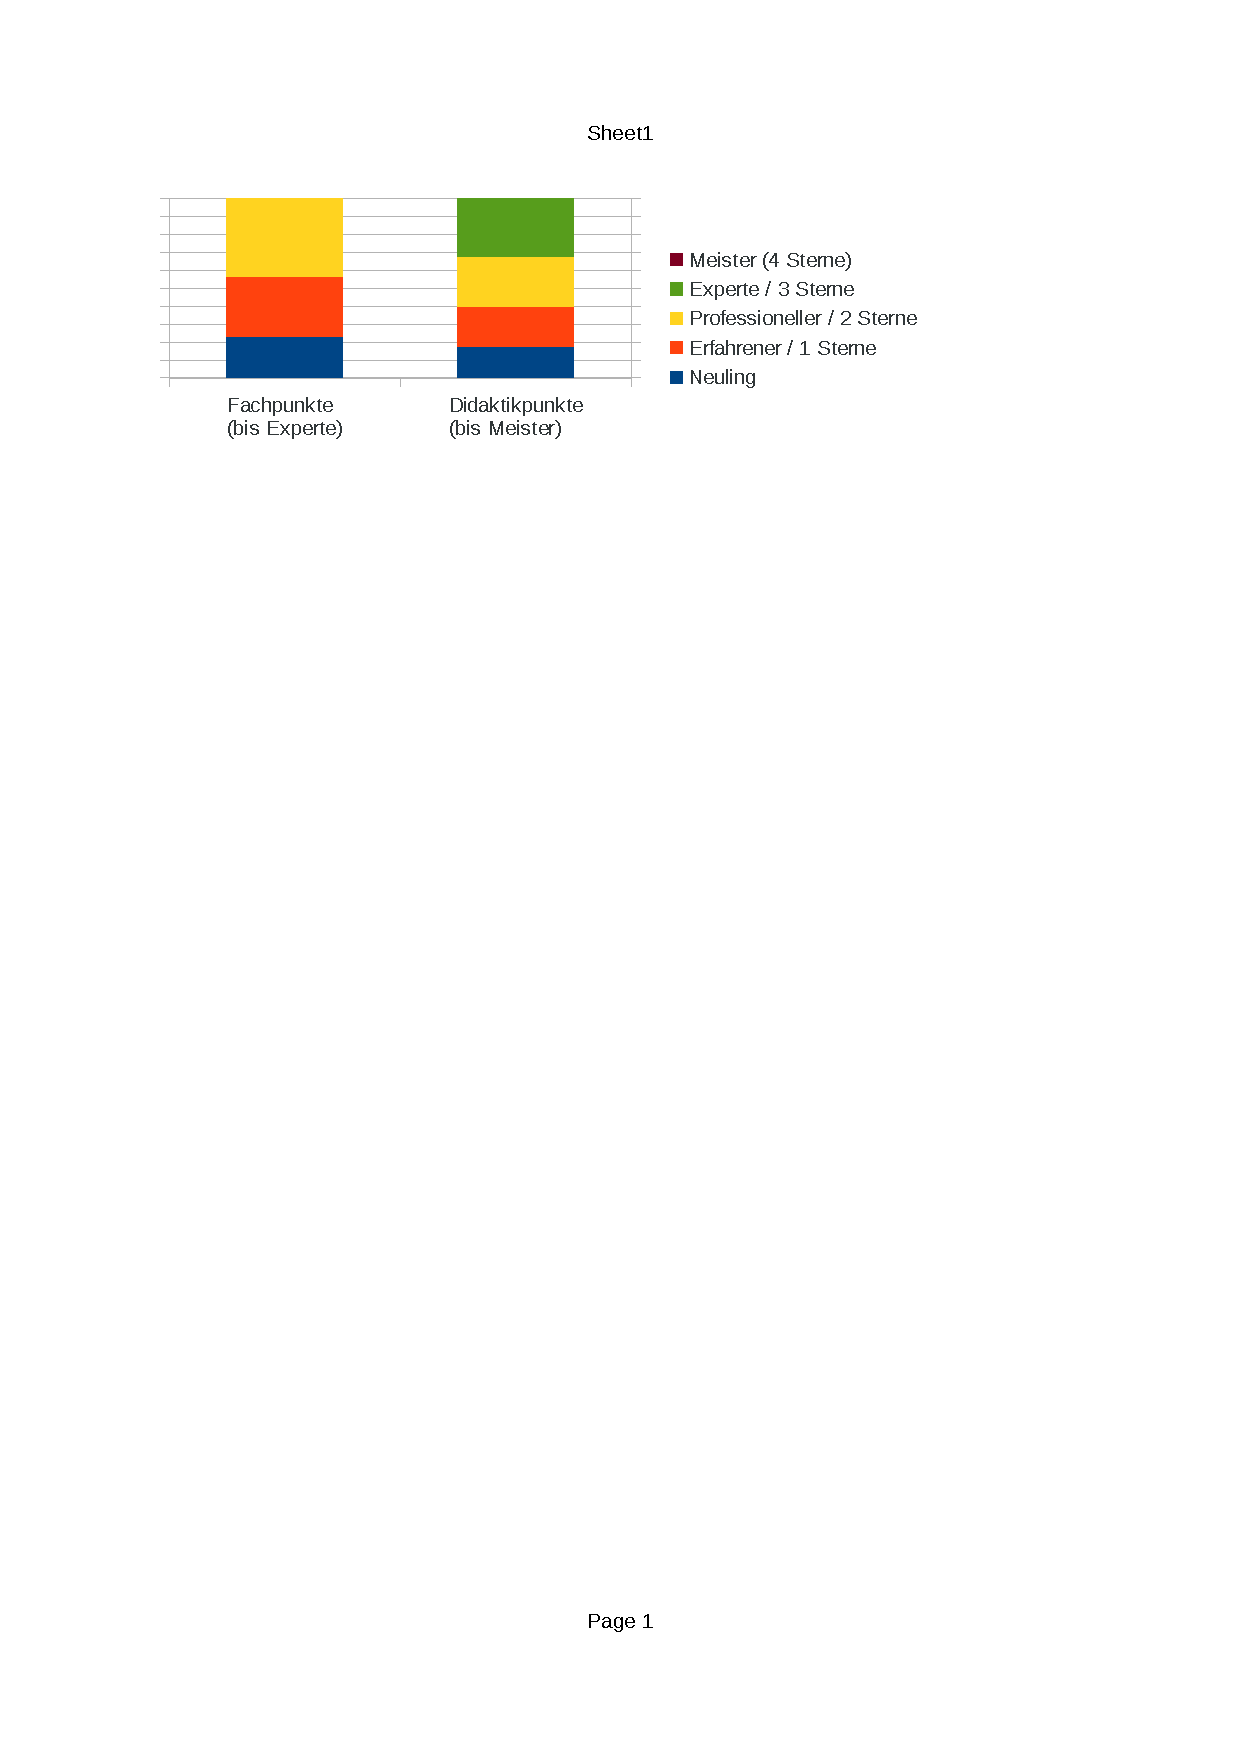
\includegraphics[width=1\textwidth]{verteilungDerPunkte.png}
\caption{Verteilung der Punkte}\label{ref:vertPunkt}
\end{figure}
Ein Meister hat durch das Erhalten der höchsten Wertung für die didaktische
Fähigkeit bereits bewiesen, dass er Spaß an der Vermittlung von Wissen hat.
Demnach bedarf er keiner weiteren Motivation eines höheren Ranges.
Vielmehr möchte er keine negativen Bewertungen seiner Lernenden erhalten und
bemüht sich der weiteren hochwertigen Qualität seiner Lerneinheiten.

\section{Rollen für Anwender}
Passend zum zuvor beschriebenen Konzept werden drei Rollen für Anwender
definiert. Dabei ist das Innehaben mehrerer Rollen zur gleichen Zeit ein Teil
des Modells. Zusammenfassend sind die Rechte und Pflichten eines Nutzers in den
verschieden Rollen in Tabelle \ref{tab:privilegesRoles} aufgeführt. Das dort
aufgeführte Forum ist nicht Teil der ersten produktiven Version (siehe
Abschnitt \ref{ref:weitereIdeen})

\subsection{Administrator}
Der Administrator ist der Verwalter der Plattform und damit für den
reibungslosen Ablauf seitens der Nutzer verantwortlich. Dazu kontrolliert er den
Zusammenhalt des Systems und greift bei inkonsistenzen oder Fehlern ein. Auch
bildet er die Schnittstelle zur Community, die sich in der Weiterentwicklung von
Masterly Mate engagiert.

\subsection{Lernender}
Der Lernende bildet die Hauptzielgruppe des Systems. Er soll WBTs finden, diese
durcharbeiten können und sich an Tutoren wenden, falls er auf ein Problem oder
Unklarheiten stößt. Dazu bietet Masterly Mate ihm das auffinden eines an sein
Fachwissen angepasstes Training. Weiterhin kann er Tutoren kontaktieren, die in
seinem Umkreis wohnen und passend zu seinem Rang Inhalte zu erläutern verstehen.
Die Lokation wird anhand der Postleitzahl festgemacht.

Ein Lernender kann in seinem fachlichen Level bis zum Experten aufsteigen.
Nähere Erläuterungen zu den fachlichen Rängen wurden in Abschnitt
\ref{ref:rankTopic} aufgeführt.

\subsection{Tutor}
Ein Lernender kann ab dem zweiten fachlichen Rang des Dreyfus-Modells (siehe
\ref{ref:dreyfus}) in seinem Profil die Einstellung "`Tutor"' anwählen. Damit
erscheint er unter den Suchergebnissen für Lernende, die einen Tutor suchen. Als
Tutor wird man von Lernenden gefunden, die Unterstützung in einem Fachgebiet
suchen.

\section{Dokumentation der API}\label{ref:archDoc}
RoR bietet ein Werkzeug, welches automatisch eine API-Dokumentation der
Anwendung erstellt. Mit der Kommandozeile \textit{rake doc:app} wird dies
realisiert. Dabei ruft rake\footnote{Kurzwort für Ruby Make} im Namespace doc:
die Funktion app auf, die neben guides und rails die Dokumentation für die
eigene Applikation erstellt. Dabei werden die Kommentare
aus dem Quelltext verwendet, um eine übersichliche Darstellung der
programmierten Funktionen zu schaffen \cite{edgeGuide:2013}.

\section{Automatisch generierte Filterung von Ergebnissen}\label{ref:autoResult}
\begin{k}
@Benni
\begin{itemize}
  \item Profilinfos werden ausgelesen und zur Eingrenzung der Ergebnisse
  verwendet
  \item daher kein Suchfeld nötig
\end{itemize}
\end{k}
Die Suche von WBTs wird Über reine SQL-Abfragen realisiert. 
Dies bedeutet, dass bei einem Aufruf der WBT-Liste, die Daten des betreffenden Users ausgelesen werden. 
Entsprechend des Levels eines Users im betreffenden Themengebiet werden die
Dafür vorgesehenen WBTs, welche er noch nicht absolviert hat angezeigt. 

\section{Themen}
Die Themen (oder Topics/Themengebiete) grenzen die WBTs voneinander ab und sind
neben den Leveln ein Suchkriterium. Jedes WBT ist Teil mindestens eines
Themengebietes. Außerdem sind die Ränge an die Themen gebunden. Der Benutzer
kann WBTs in jedem Themengebiet absolvieren und im Rang aufsteigen. Dabei ist zu
beachten, dass ein Benutzer einen bestimmten Rang nur in einem Themengebiet
haben kann. Das bedeutet, dass er zwar in einem Gebiet den Status eines
Expertise haben kann, in einem ganz anderen jedoch ein absoluter Newbie ist. Ist
ein WBTs zwei (oder mehr) Themen zugeordnet, so erhält der Benutzer bei
Abschluss die Punkte für beide Themengebiete. Themen können Unterthemen haben,
daher kann ein Benutzer innerhalb eines Überthemas unterschiedliche Ränge haben.
So kann z.B. ein Benutzer im Thema Informatik ein Expertise sein und zugleich in
den Unterthemen Datenstrukturen und Algorithmen Specialist bzw. Newbie sein.
Die Beziehung von Benutzer zu Themengebiet ist m:n, ebenso ist die Beziehung
zwischen Thema und WBT m:n. Die Beziehung von Themen zu ihren Unterthemen ist
1:n. Das hier Beschriebene ist der Stand der Alpha-Version. Eine mögliche
Änderung für die Zukunft wäre, dass erreichte Punkte eines Unterthemas auch im
Überthema gutgeschrieben werden.
	\chapter{Anwenderseite}
Dieses Kapitel zeigt den Teil der Konzeption, der für Anwender sichtbar und
wichtig ist.

\section{Gamification}\label{ref:gamificationConcept}
In Abschnitt \ref{ref:gamification} wurden die wesentlichen Aspekte von
Gamification angesprochen. Hier erfolgt die Konkretisierung derartiger
Eigenschaften in die Konzeption von Masterly Mate.

\subsection{Belohnungskriterien}
Um die Motivation stets auf einem hohen Niveau zu halten, bedient sich Masterly
Mate einer Auswahl an Belohnungskriterien.

Die \textbf{erreichte Punktzahl} im Quiz eines WBTs wird für das Erreichen des
nächst höheren Levels hinzugenommen. Analog dazu erhalten Tutoren
\textbf{Sterne} für qualitativ hohe Unterweisungen. Zuzüglich zu den regulären
Punkten für die fachlichen und den tutoriellen Rang können \textbf{Wertmarken}
gesammelt werden mit denen einem Avatar oder dem \ac{GUI} mehr
Gestaltungsmöglichkeiten verliehen werden.

\subsection{Etappenweise Herausforderungen}
Ein weiteres Mittel, um die Motivation zu fördern sind Spielmechaniken, die in
die Anwendung eingebracht werden. Für diese ist es erforderlich, dass für jede
Art von Nutzer Anreize bestehen. 

Die drei Ränge Neuling, regulärer Nutzer und Enthusiast sind nicht zu
verwechseln mit den Rängen des Dreyfus-Modells aus Abschnitt
\ref{ref:dreyfusConcept}. Die hier betrachteten Ränge in Bezug auf Gamification
berücksichtigen die Handhabe der Software als solche. Ein Neuling verwendet die
Anwendung zum ersten mal oder bisher nur wenige male. Der reguläre Nutzer ist
ein Stammgast der Plattform, während der Enthusiast schier nicht schlafen kann,
ohne die Anwendung täglich verwendet zu haben.

Allen Nutzern ist gemeinsam, dass sie sich selbst gut evaluieren können. Sie
erhalten die Möglichkeit Statistiken einzusehen. Für die erste Version von
Masterly Mate ist eine Art Ladebalken vorgesehen, welcher je nach Füllstand
zeigt, wie groß die Erfüllung der erforderlichen Gesamtpunktzahl für einen Rang
ist. Über seine Wertung kann sich ein Nutzer stets im Feld aller Nutzer
einordnen. Dabei kann jeder für sich individuell entscheiden, ob es für ihn
wichtig ist, in die Top-Ten zu gelangen \cite{grubenMerkeBabics:2012}.

\subsubsection{Neuling}
Als erstmaliger Nutzer einer Plattform oder Anwendung benötigen Neulinge einen
vereinfachten Einstieg und eine leicht verständliche Anleitung. Auch muss die
GUI übersichtlich gestaltet sein, sodass nicht bereits nach wenigen Klicks
Frustration entsteht.

In Masterly Mate wird daher von Beginn an eine Möglichkeit zur
Internationalisierung (siehe Abschnitt \ref{ref:internationalisierung})
umgesetzt. So sieht der Anwender das Interface stets in seiner Sprache der Wahl
und stößt somit nicht auf Verständnisprobleme.

Weiterhin erhält ein neuer Nutzer analog seines fachlichen Rangs Zugang zu
einfachen WBTs, die leicht verständlich sind. Stößt er hier bereits auf
Probleme, so kann er sich einen Tutor zu Rate ziehen
\cite{grubenMerkeBabics:2012}.

Eine Anleitung im Sinne eines Handbuches ist für die erste produktive Version
nicht angedacht.
  
\subsubsection{Regulärer Nutzer}
Nutzer, die die Anwendung in moderater Weise nutzen, sind grundsätzlich
zufrieden mit dem, was ihnen geboten wird. Sie sind aber noch
begeisterungsfähig.

Ein solcher Stammgast kann in Masterly Mate auf noch höhere Ränge aufsteigen,
denn ihm fällt es leichter den in Abschnitt \ref{ref:rankTopic} angesprochenen
jährlichen Test zu bestehen. Als Tutor strebt er eventuell danach ein Meister zu
werden.

Um ein Erlebnis analog des in Abschnitt \ref{ref:basFlow} beschriebenen Flows zu
unterstützen, steigt auch das Niveau der zur Verfügung stehenden WBTs. So kann
der Stammnutzer bei Bedarf stets neue Herausforderungen suchen
\cite{grubenMerkeBabics:2012}.

\subsubsection{Enthusiast}
Ein Enthusiast wird alles daran setzen seinen Experten oder meisterlichen Rang
zu behalten. Er wird also weiterhin Unterweisungen geben und genießt sein
Privileg, WBTs editieren zu können. Je nach Interesse kann er seinen Meister
Rang dazu nutzen in andere Fachgebiete einzusteigen und dort für sämtliche
Mitglieder unterhalb seines zugehörigen fachlichen Rangs mit Rat zur Seite zu
stehen \cite{grubenMerkeBabics:2012}.

\section{Generieren von Motivation}
Zusammen mit der im vorangegangenen Abschnitt beschribenen Konzeption von
Gamification in Masterly Mate wird an dieser Stelle die Integration der in
Abschnitt \ref{ref:basMotivation} beschriebenen Motivation erläutert.

In diesem Abschnitt wird ein Blick auf die motivierenden Merkmale aus
Anwendersicht beschrieben, die im Wesentlichen bereits im vorangegangenen
Abschnitt für die Umsetzung von Gamification besprochen wurden. Dieser wird
separiert in intrisische und extrinsische Motivation dargestellt.

\subsection{Intrinsisch motivierende Aspekte}
Ein Nutzer von Masterly Mate strebt von sich aus nach Weiterbildung und damit
nach einem höheren fachlichen oder didaktischen Rang. Beinahe nebenbei steigt er
dafür immer tiefer in fachliche Themen ein. Für seine Leistungen möchte er
Feedback erhalten und mit gleichgesinnten reden oder helfen. 

Tutoren haben zusätzlich die Möglichkeit ihr Langzeitgedächtnis mithilfe von
immer wiederkehrenden Unterweisungen zu schulen. Damit zusammenhängend
trainieren sie sich in ihren didaktischen Fähigkeiten.
  
\subsection{Weitere extrinsisch motivierende Merkmale}
Zu den intrinsischen Motivatoren kommen weitere extrinsische Motivatoren. Dazu
gehören der Erhalt von Belohnungen, mehr Möglichkeiten in der Gestaltung des
Interfaces oder Avatars oder eine Bestenliste zum Leistungsvergleich mit anderen
Nutzern.

Macht man sich in der Plattform einen Namen als Tutor oder beteiligt sich an
regen Diskussionen im Forum, so erfährt man Lob und Kritik von gleichgesinnten.
Insgesamt lässt Masterly Mate eine persönliche Analyse in Form von Statistiken
zu.
	\part{Implementierung}
	\chapter{Entwurf}\label{ref:chaptScript}
Der in diesem Kapitel beschriebene Entwurf zeigt konkret, wie das Konzept von
Masterly Mate umgesetzt werden wird. Hier werden Schemata und Architekturen
entwickelt, die im Kapitel \ref{ref:chaptImplementation} in Programmcode
umgesetzt werden.

\section{Realisierungsmethodik}
Nachdem in den vorangegangenen Kapiteln das Konzept von Masterly Mate erläutert
wurde, stellt sich die Frage nach einer geeigneten Möglichkeit zur Umsetzung. Da
die Anwendung stets verfügbar, leicht erreichbar, modular und einfach zu
verwalten sein soll, ist \ac{RoR} das Mittel der Wahl. Dieses bietet viele
interessante Features in Form von sogenannten gems, die dank einer regen
Community stets aktualisiert und erweitert werden. Zudem unterstützt es moderne
Programmierparadigmen, wie \ac{DRY} und \ac{KISS}. Dadurch bleibt die Anwendung
aus Sicht der Programmierer übersichtlich und erscheint sehr strukturiert. Das
das Framework der \ac{MVC}-Architektur folgt, schafft einen weiteren Grundstein
zur Trennung von Zuständigkeiten\footnote{bekannter unter "`separation of
concerns"'} und sorgt auch damit für Übersichtlichkeit. 

Weiterhin ist dieses Framework für die Weiterentwicklung im
OpenSource-Bereich prädistiniert, da damit bisher populäre
Webanwendungen, wie Twitter, realisiert wurden.

Darüber hinaus wird darauf geachtet, die Komponenten nach und nach nur dann zu
entwickeln, wenn sie tatsächlich gebraucht werden. Diese Vorgehensweise nach dem
\ac{YAGNI}-Prinzip beugt ein überlaufenes, unübersichtliches und schwer
zu wartendes Produkt vor.

\section{Internationalisierung}\label{ref:internationalisierung}
Die Internationalisierung gewährleistet eine Webanwendung, die möglichst
unabhängig von natürlichen Sprachen ist. Die Internationalisierung wird auch bei
Masterly Mate weitestgehend bereits in der ersten Version eingesetzt.
Die RoR API bietet dafür die Klasse I18n an, mit dessen Hilfe die
Internationalisierung durchgeführt werden kann. Die Bezeichnung I18n
kennzeichnet den Begriff Internationalisierung als Numeronym. Die Zahl 18 steht
für die Anzahl an Buchstaben, die zwischen den Buchstaben I und n liegen.
Die Klasse I18n bietet neben vielen anderen Methoden eine essentielle Methode
an, mit dessen Hilfe die Internationalisierung von Masterly Mate weitestgehend
realisiert werden kann. Die Methode trägt die Bezeichnung t als Kurzform für
translate. Diese Methode erwartet als einzigen Parameter eine Zeichenkette,
welche den Pfad zu dem entsprechenden Sprachstring angibt. Bei der
Initialisierung der RoR Anwendung Masterly Mate, werden sämtliche *.yaml Dateien
aus dem Verzeichnis config/locales/ als Sprachdateien geladen. Der Name einer
Sprachdatei sollte aus Konventionsgründen einer Rails Webanwendung, stets den
Ländercode beinhalten. In der ersten Version von Masterly Mate werden die
Sprachen Deutsch und Englisch unterstützt. Sven Fuchs bietet für sämtliche
Sprachen auf
Github\footnote{\url{https://github.com/svenfuchs/rails-i18n/tree/master/rails/locale}}
vorgefertigte Sprachdateien an. Diese Sprachdateien definieren für die jeweilige
Sprache entsprechende Formatierungen, wie z.B.
Datum- und Zeitangaben. Aber auch die Werte für Labels von
Formularsteuerungskomponenten, wie z.B. die Submit-Schaltfläche, werden in
diesen Sprachdateien festgelegt. Die anwendungsspezifischen Strings müssen
selbstverständlich selbst in *.yaml Sprachdateien definiert und im Verzeichnis
config/locales/ abgelegt werden. Eine RoR Sprachdatei ist hierarchisch
aufgebaut. Die einzelnen Hierarchieebenen werden dann später beim Zugriff auf
ein Sprachstring über ein Punkt voneinander getrennt. Grundlegend definiert man
eine von der natürlichen Sprache unabhängige Zeichenkette dadurch, indem ein
fester Bezeichner gefolgt von einem Doppelpunkt definiert wird. Nach dem
Doppelpunkt folgt die sprachabhängige Zeichenkette. Im Programmcode wird an den
Stellen, an denen eine sprachenunabhängige Zeichenkette ausgegeben werden soll,
die Methode t der Klasse I18n eingesetzt und dieser als Parameter der Pfad zu
dem entsprechenden Bezeichner übergeben.
Masterly Mate ist nahezu vollständig für die Sprachen Deutsch und Englisch
Internationalisiert. Lediglich die von den Nutzern erstellten WBTs sind nicht
Internationalisiert. Einige WBT-Engines bieten den Mechanismus zur
Internationalisierung nicht an. Aus diesem Grund wurde dieses Vorhaben im Rahmen
dieser Studienarbeit vernachlässigt.

\section{Beschreibung des Entwurfsklassendiagramms und
Use-Case}\label{ref:classModel}

\subsection{Use-Case Diagramm}
Im obigen Use-Case Diagramm, sind die einzelnen benötigten Komponenten
enthalten, wie sie die Analyse ergeben hat. Zunächst einmal lassen sich Aktoren
ausmachen, welche in System/Software-Aktoren und menschliche Aktoren aufteilen
lassen. 

Bei den Softwareseitigen Aktoren ergab die Analyse als Aktoren den Webserver,
ein Einzelnes WBT (sie sollen nach Abschluss die Punkte im System eintragen),
das Autorenwerkzeug und den Webbrowser. Auf der Seite der Aktoren ließe sich der
Lernende (Standard-User), Tutor, Autor und Admin ermitteln. Zu beachten ist,
dass die Aufteilung der menschlichen Aktoren auch eine Berechtigungshierarchie
darstellt, wobei ein Lernender die geringsten und ein Admin die meisten
Berechtigungen hat.

Die einzelnen Use Cases werden nun jeweils im folgenden kurz beschrieben. Zu
beachtenn ist dabei noch, dass diese Analyse sich nicht zwingend mit dem
Ergebnis aus der Studienarbeit deckt, da Funktionalitäten auf spätere Releases
verschoben worden sind.

\subsubsection{WBT durcharbeiten} 
Agierende Aktoren: \begin{itemize}
  \item WBT
  \item Lernender
  \item Tutor
  \item Autor
  \item Admin 
\end{itemize}

Ein Benutzer startet ein WBT und schließt es erfolgreich ab bzw.
scheitert oder beendet es vorzeitig. Im Anschluss daran, werden die erreichten
Punkte im System eingetragen. In der Version der Studienarbeit, wird dies noch
vom Benutzer selbst durchgeführt. Später soll dies das WBT übernehmen.
	
\subsubsection{Bewerten}
Agierende Aktoren: \begin{itemize}
  \item Lernender
  \item Tutor
\end{itemize} 

Den Use Case Bewerten gibt es in zwei Ausprägungen. Die erste Ausprägung ist die
Bewertung eines Tutors. Hat ein Lernender oder eine anderer Tutor (im folgenden
beide als "Lernende" bezeichnet) von dem Betreffenden Benutzer Hilfe erhalten,
so kann der Lernende im Anschluss daran diese Hilfe im System bewerten.
Dies kann er mit Sternen und wahlweise mit einem Kommentar tun (Kommentar noch
nicht in der Alpha-Version). Die Zweite Ausprägung ist die Bewertung eines WBTs.
Ein Benutzer muss das WBT dafür abgeschlossen haben. Ebenso wie beim Tutor kann
er dies über Sterne und Kommentare tun.
	
\subsubsection{Sprache verwalen}
Agierende Aktoren: \begin{itemize}
  \item Alle menschlichen Aktoren (Ausprägung Sprache
hinzufügen kann nur der Admin)
\end{itemize}

Ebenso wie im obigen Use Case gibt es hiervon zwei Ausprägungen.
Nummer Eins ist der Use Case Sprache wechseln. Dieser kann von jedem Benutzer
durchgeführt werden und bewirkt, dass alle Zeichenketten in MasterlyMate, welche
in der betreffenden Sprache vorhanden sind, ausgetauscht werden. Use Case Nummer
Zwei kann nur von einem Administrator durchgeführt werden. Und bewirkt die
Erzeugung einer weiteren Sprache, welche eingestellt werden kann. Gegenwärtig
wird dies noch direkt durch eine Änderung der Sprachdateiten getan.

\subsubsection{Profil verwalten}
Agierende Aktoren: \begin{itemize}
  \item Alle menschlichen Aktoren
\end{itemize}

Auch dieser Use Case verfügt über zwei Ausprägungen. Der erste Use Case ist das
bearbeiten eines Profils. Dies kann nur der besitzer des jeweiligen Profils.
Den anderen Use Case kann hingegen jeder Benutzer durchführen. Es handelt sich
dabei um das Betrachten eines Profils. Dies ist insbesondere für die
Kontaktaufnahme eines Benutzers zu einem Tutor notwendig.

\subsubsection{Suchen}
Agierende Aktoren: \begin{itemize}
  \item Alle menschlichen Aktoren
\end{itemize}

Es können sowohl Tutoren als auch WBTs gesucht werden. Dabei wird jeweils
berücksichtigt welches Themengebiet gefragt ist.
	
\subsubsection{Themengebiet abfragen}
Agierende Aktoren: \begin{itemize}
  \item Webserver
\end{itemize}

Der Webserver überprüft bei einer Suchanfrage die einzelnen Themen.
	
\subsubsection{Themen verwalten}
Agierende Aktoren: \begin{itemize}
  \item Admin
  \item Webserver
\end{itemize}

Nur der Admin kann die beiden Ausprägungen dieses Use Cases durchführen, welche
das Hinzufügen und Löschen eines Themas darstellen.
	
\subsubsection{WBT verwalten}
Agierende Aktoren: \begin{itemize}
  \item Admin
  \item Autor
  \item Webserver
\end{itemize}

Dieser Use Case besitzt drei Ausprägungen. Admin und Autor können WBTs
einbinden. Es kann jedoch nur der User, welcher ein WBT eingebunden hat, dieses
auch wieder entfernen bzw. ersetzen. Dies gilt nicht, wenn der betreffende
Benutzer ein Administrator ist. Dieser kann jedes WBT löschen oder ersetzen.
	

\subsection{Entwurfsklassendiagramm}
In dem Entwurfsklassendiagramm, sind die Models und ihre Beziehungen zueinander
dargestellt. Diese Modelle bilden einzelne Konzepte im System ab. So stellt User
ein Zentrales Modell dar, welches als Abbildung eines Benutzers im System für
die Authentifizierung verantwortlich trägt. Außerdem werden dem User
verschiedene Themen und WBTs zugeordnet. Diese Verbindungen benötigen jeweils
Assoziationsklassen. Dies liegt daran, dass es in dieser Verbindung Attribute
gibt, welche sich nicht eindeutig User oder WBT bzw. Thema zuordnen lassen. Bei
der Verbindung User-Thema benötigt man ein Attribut für die Punkte, welche
bisher von dem User in dem System erziehlt worden sind. Außerdem muss klar sein
welchen Rang ein User in dem jeweiligen Thema inne hat. Die Verbindung User-WBT
dagegen benötigt eine Variable um zu hinterlegen ob ein User das WBT bereits
einmal abgeschlossen hat und wenn ja, wie viele Punkte er erreicht hat. Im folgenden
wird auf die Modelle des UML-Diagrammes näher eingegangen. Dazu sei noch
angemerkt, dass zwischen einem realen Konzept und dem des Models underschieden
wird. D.h. wenn z.B. im Folgenden vom User die Rede ist, dann ist hierbei das
Model oder eine Instanz der User-Klasse gemeint. Wird hingegen vom Benutzer
gesprochen, so ist auch tatsächlich jener gemeint.  

\subsubsection{WBT}\label{ref:objectWBT}
Das WBT-Model verfügt über eine ID, sowie über einen Pfad zur eigentliche
SCORM-Datei. Wie bereits erwähnt ist es einem oder mehreren Themen (Topics)
zugeordnet. Auf Datenbankseite bedeutet dies, dass eine Zwischenentität zwischen
Topic und WBT eingeführt werden muss. 

\subsubsection{Topic}
Im UML-Diagramm ist ersichtlich, dass das Model Topic eine referenz auf sich
selbst besitzt. In dieser Referenz kann ein Topic sowohl die Rolle des über- als
auch des Unterthemas bekleiden. Unterthemen dienen einer genaueren Unterteilung
der WBTs. Tobics werden mit ihrem Namen identifiziert. Dies gilt auch für die
übergeordneten Topics. Dies bedeutet, dass ein Unterthema die Information
besitzt, zu welchem Topic es gehört. Diese vorgehensweise ist auch für die
Datenbank hilfreich, da so der Maxime entsprochen wird, den Fremdschlüssel auf
der N-Seite zu notieren.

\subsubsection{User}
Das Dritte große und wahrscheinlich sogar größte Model ist der User. Er ist
gekennzeichnet durch einen Benutzernamen, Vor- und Nachname, Passwort,
Geburtstag und einer Email-Adresse. Der User, stellt die Benutzer im System dar.
Er wird für die Registrierung und Authentifizierung verwendet. Des Weiteren
werden ihm die Punkte zugeordnet, welche ein Registrierter Benutzer in einem WBT
erzielt. Damit werden ebenso die Ränge dem Benutzer zugeordnet, von welchen er
beliebig viele haben kann (siehe dazu Model: Ränge). 
Ein Benutzer ist außerdem in einer oder mehrerer der möglichen Gruppen
eingeordnet.
Über diese wird geregelt, welche berechtigungen er im System hat. Näheres dazu
ist im entsprechenden Abschnitt zu finden.
Eine besondere Funktion fällt der Zuordnung eines User zu einer Location zu. Mit
ihr ist es möglich, dass Benutzer Tutoren in der Nähe ihrer eigenen Wohnstätte
finden können (Auch dazu, sie im entsprechenden Abschnitt).

\subsubsection{Group}
Die Gruppen werden zur Festlegung der Berechtigungen verwendet. Ein User
kann in beliebig vielen Gruppen sein und diese wiederum kann beliebig viele User
enthalten. Die Gruppen im System sind die Administratoren, welche volle Rechte
im System besitzen. Die etwas schwächeren Tutoren können WBT hochladen und ihr
eigenes löschen. Außerdem können sie von anderen Usern bewertet werden. Die
Dritte vorhandene Gruppe sind die normalen User. Diese können lediglich WBTs
durcharbeiten, Profile von anderen Usern einsehen, sowie ihr eigenes bearbeiten.
Implizit vorhanden, jedoch nicht implementiert sein soll die Gäste-Gruppe. Diese
umfasst alle Benutzer, welche keinen User im System besitzen.

\subsubsection{Location}
Eine Location beschreibt den groben Standort an dem ein Benutzer wohnt. Daher
verfügt dieses Model auch nicht über die kompletten Adressdaten eines Benutzers,
sondern nur über die Stadt, die Postleitzahl sowie das Land. Da die Location
einzig den Sinn hat, die Suche nach geeigneten Tutoren einzugrenzen ist eine
genauere Standortsbestimmung nicht notwendig. Da es mehrere User gegen kann, die
der gleich Location zugeordnet sind, ist wird diese auf der User-Seite durch die
entsprechende ID der Location identifiziert. 

\subsubsection{Assessment}
Das Assesment bildet als Assoziationsklasse zwischen User und Topic die
Beziehung zwischen dem User und einem Topic ab. In ihr wird gespeichert, wie
viele Punkte er durch die Absolvierung von WBTs in einem Thema erreicht hat.
Entsprechend zeigt das Assesment auch den Rang an, den ein Benutzer in einem
bestimmten Thema erreicht hat.

\subsubsection{Rank}
Der Rang eines Benutzer spiegelt den Erfahrungsstand wieder, den ein Benutzer in
einem Thema erreicht hat. Er wird bei entsprechender Punktzahl (Erspielte Punkte
bzw. Sterne) vom System vergeben.

\section{Funktionalitäten aus Nutzersicht}
Prinzipiell ist Masterly Mate aus zwei Komplexen aufgebaut. Zum einen kann sich
ein Nutzer fachlich weiterbilden. Zum Anderen bietet ein Nutzer als Tutor seine
Hilfe für ein bestimmtes Fachgebiet an.

\subsection{Masterly Mate für Lernende}
Aus Sicht der Lernenden baut sich Masterly Mate aus den folgenden Komponenten
auf.

\subsubsection{Registrieren und Einloggen}
Ein neuer Nutzer wird sich zunächst registrieren. Ist dies bereits geschehen,
kann er sich einloggen und sich dem Bearbeiten von WBTs oder der Administration
seines Profils widmen.

\subsubsection{Durcharbeiten von WBTs}
Ist ein Nutzer an Weiterbildungsangeboten interessiert, so geht er ein oder
mehrere WBTs durch. Dazu erhält er nach einer passenden Filterung der Ergebnisse
anhand einer Themenwahl und des dazugehörigen fachlichen Ranges (siehe Abschnitt
\ref{ref:autoResult}) eine verfügbare Liste an WBTs, die er nach seinem Gusto
bearbeiten kann.

\subsubsection{Tutorensuche}
Stößt der Lernende beim Durcharbeiten von WBTs auf ein fachliches Problem, so
kann er einen Tutor aufsuchen. Die Darbietung passender Tutoren erfolgt ebenso
nach einer automatischen Filterung. Die Filterung wird auch hier anhand des
fachlichen Rangs des Lernenden und des Themengebiets vorgenommen. Hinzu kommt
der didaktische Rang des Tutoren und die jeweils angegebene Postleitzahl
Lernenden und des Tutors, sodass ein Treffen aufgrund der räumlichen Nähe
einfacher möglicht wird.

\subsubsection{Profil administrieren}
Jedem Nutzer ist es erlaubt, sein eigenes Profil zu administrieren. Dort kann er
sein Profilbild und andere persönliche Angaben, wie Spitzname, Name und
Postleitzahl ändern. Zusätzlich kann er hier eine Option anhaken, die ihm zum
Tutor macht. Damit erscheint er für andere Lernende in den Suchergebnissen für
passende Tutoren. Demgegenüber kann er den Haken wieder entfernen, falls er kein
Tutor mehr sein möchte.

\subsubsection{Navigation, Impressum, Kontakt}
Eine übersichtliche und nicht zu detailierte Navigation für Masterly Mate war
ebenfalls ein Ziel dieser Studienarbeit. Die Funktionsweise eines
Navigationsmoduls sollte nicht neu entwickelt werden. Aus diesem Grund wurden
einige vorgefertigte Gems für die Navigation in Betracht gezogen. Das Gem,
welches letztlich für die Navigation in Masterly Mate eingesetzt wurde, nennt
sich Simple-Navigation\footnote{\url{https://github.com/andi/simple-navigation}}.
Die Handhabung dieses Gems ist sehr einfach und darüber hinaus bietet es eine
übersichtliche Infrastruktur und somit ein Grundkonzept für die Funktionsweise
einer Navigation. Die Elemente der Navigationsleiste werden an einer zentralen
Stelle in der config/navigation.rb definiert. Auch das Festlegen von
Subelementen ist möglich. Weiterhin kann man eine von mehreren 
Darstellungsarten, wie z.B. einer ungeordneten HTML Liste, Linklisten,
Breadcrumbs, etc. für das Navigationsmoduls auswählen. Für Masterly Mate wird
eine entsprechend mit CSS formatierte Linkliste eingesetzt.
Für das Impressum wurde im Rahmen dieser Studienarbeit keine eigene Seite in der
Webanwendung vorgesehen. Dieses befindet sich daher in der Fußleiste von
Masterly Mate. Auch ein Kontaktformular wurde in dieser Arbeit nicht vorgesehen.
Der Kontakt erfolgt in der aktuellen Version über das Anschreiben an die
Entwickler von Masterly Mate per E-Mail. 

\subsubsection{Themen}
Themen fungieren für den Benutzer zum Einen als Suchfilter bei der Suche nach
den WBTs. Dies sorgt dafür, dass der Benutzer ohne umschweife auf WBTs zugreifen
kann, welche für ihn interessant sind. Außerdem dienen Themen dazu, die
unterschiedlichen Ränge, welche ein Benutzer zur selben Zeit in Masterly Mate
haben kann, voneinanderabzugrenzen. Jeder Benutzer kann in einem Thema nur genau
einen Rang inne haben. Umgekehrt kann er jedoch in beliebig vielen Themen einen
Rang haben.

Zu diskutieren ist, hierbei ob ein Benutzer jeweils in einzelnen Unterthemen
einen Rang inne hat und auch im Oberthema oder nicht. Wenn er in jedem wirklich
Thema einen Rang inne haben kann ist außerdem zu klären, wie sich das auf den
Rang im Überthema auswirkt. Er könnte in diesem Falle sowohl die erzielten
Punkte gutgeschrieben bekommen als auch in allen darüberliegenden Themen. Dann
hätte er in dem Überthema einen Rang, welcher mindestens so hoch ist, wie der
höchste Rang in einem der Unterthemen. 
In einem anderen Falle, namentlich Ränge in allen Themen ohne das kaskadieren
der Punkte, wäre es möglich, dass der Benutzer in einem Unterthema Meister sein
könnte im Übergeordneten jedoch nur Erfahrener, da er in dem Überthema nur die
Punkte erhält, welche direkt diesem Thema untergeordnet sind.
Ein ganz anderer Fall hingegen wäre es, wenn der Benutzer nur in einem der
Überthemen einen Rang haben könnte und die Unterthemen einzig und allein der
Unterteilung dienen. In diesem Falle müsste man im Datensatz nachprüfen ob das
Thema, zu dem das abgeschlossene WBT gehört, ein übergeordnetes Thema hat. Ist
dies der Fall so müssten dieses Thema überprüft werden. Dieser Vorgang müsste
solange fortgesetzt werden, bis das hierarchisch höchste Thema gefunden ist.
In diesem Thema würden dann die Punkte dem Benutzer zugeteilt.

Ein ganz anderes Problem stellt das löschen von Themen dar. Auch hier gibt es
mehrere Möglichkeiten. So ist es denkbar, dass bei einer Löschung eines Themas,
alle Unterthemen mit WBTs gelöscht werden. Dies sollte allerdings mit Vorsicht
genossen werden und am besten mit einer oder eventuell zwei Abfragen hinterfragt
und bestätigt werden.
Eine andere, weniger gefährliche Option wäre es, die enthaltenen Unterthemen und
WBTs dem übergeordneten Thema des gelöschten Themas zuzuordnen. In diesem Fall
ist es notwendig ein Root-Thema zu definieren, welches alle Themen beinhaltet.
In diesem Falle könnte es allerdings Themen geben, die nur in dem Root-Thema
enthalten sind. D.h. es müsste möglich sein in diesem Thema einen Rang
zu erhalten (Man könnte sich an dieser Stelle fragen ob es nicht Sinvoll wäre,
dort ein WBT zur "`frage nach dem Leben, dem Universum und Allem"' zu
platzieren, weiter sei die Frage erlaubt, ob ein Meister in diesem Thema sich
``Master of the Universe'' zu nennen habe). Alternativ könnte man abfragen ob
ein WBT sich nur innerhalb des Root-Themas befindet und wenn dies der Fall ist,
dem Benutzer den Zugriff verwehren.  

\subsection{Masterly Mate aus Sicht eines Tutors}
Ein Tutor ist quasi eine erweiterte Form eines Lernenden. So bleiben dem Tutor
die verfügbaren Möglichkeiten eines Lernenden erhalten. Hinzu kommen zwei
weitere Funktionen.

\subsubsection{Lernende unterstützen}
Lernende werden gelegentlich an ihre Grenzen stoßen und Tutoren zu Rate ziehen.
Als Tutor auf Masterly Mate ist man, da man sich selbst in beliebigen
Fachgebieten weiterbilden kann, mit einem Lernenden nahezu gleichgestellt. Dem
Lernenden wir damit eine Hilfe gebende Person auf Augenhöhe vermittelt. 

Im Konzept von Masterly Mate ist nur eine Hilfe der beschriebenen Art
berücksichtigt. Tutoren können sich jedoch darüber hinaus auch auf eine
beliebige andere Art an Lernende wenden, wie zum Beispiel das geben von
Workshops oder halten von Präsentationen.

\subsubsection{WBTs verbessern und hinzufügen}
Hat ein Tutor den Rang des Meisters erreicht, so ist es ihm aufgrund seiner
herausragenden didaktischen Leistungen erlaubt, bestehende WBTs zu verbessern
oder neue zu entwickeln und auf die Plattform zu laden.
	\chapter{Implementierung}\label{ref:chaptImplementation}
\section{Nutzerverwaltung}
\section{Lokationen}
\section{Suche}
\section{SCORM}

	\part{Reflexion}
	\chapter{Zusammenfassung der Ergebnisse}\label{ref:chaptConclusion}
\begin{k}
\begin{itemize}
  \item Rails unheimlich mächtig, wir sind sehr begeistert
  \item schwierig wird es bei speziellen Dingen, die dann in Ruby programmiert
  werden müssen
\end{itemize}
\end{k}
	\chapter{Fazit und Ausblick}\label{ref:chaptSummary}

\section{Ideen für weitere Versionen}\label{ref:weitereIdeen}
\begin{k}
\begin{itemize}
  \item Nutzer kann eine Liste aller WBTs sehen, die er absolviert hat
  \item Forum
  \item Durchführung von Refactorings für DRY KISS
  \item Profilbild
  \item SCORM RTE implementieren
  \item Mailerfunktionalität
  \item Investierte Zeit mit in das Konzept für Belohnungen einbringen
  \item Am Ende jedes WBT eine Wertung abgeben (zu schwer/zu leicht) -> tendiert
  eine Wertung zu stark in eine Richtung, wird das WBT dem am nächsten passenden
  Rang zugeordnet
\end{itemize}

\subsection{Gamification für Newbies}
\begin{itemize}
    \item Quick-Start Guide (Video-)Instruction, (Video-)Tutorial
    \item Statistical evaluation (Ranking)
    \item Unlock big equipments for the selected design
    \item Possibility of using a Open-ID
    \item Newsletter-Feature
    \item Self-assessment regarding to school grades
  \end{itemize}
  
 \subsection{Gamification für Regulars}
 \begin{itemize}
    \item Collections of Achievements according to the current progression
  \end{itemize}
  
 \subsection{Gamification für Enthusiasten}
 \begin{itemize}
    \item Levels
    \item Dynamic difficulty / i.e. riddles
  \end{itemize}
  
 \subsection{Weitere Möglichkeiten für Gamification}
\begin{itemize}
\item Design Selection (Tamagochi, Avatar)
  \item Assistance possible
  \item Progress bar
  \item status message
  \item discussion room
  \item class room
  \end{itemize}
  
wie schaut das Gamification-Konzept von MM aus? Irgendwie ist Fortschrittsbalken
und Statistik und Möglichkeit als Tutor zu gering bis Meister. Gut ist der
Anreiz, ab Meister WBTs einbringen und editieren zu können. Wie war das mit dem
Avatar oder der UI, die immer besser gestaltet werden kann?

\end{k}

\section{Anschließende Vorhaben}
\begin{k}
sehen, was wird
\begin{itemize}
  \item wirklich nur in Ausnahmefällen eine DE? (siehe
  \ref{ref:blendedLearning})
  \item (un)populär
  \item neue Verwendungszwecke
  \item nur eine Installation oder mehrere
\end{itemize}

kann mithilfe von Masterly Mate ein idealer Lehrer gefunden werden?
\end{k}
	
	\phantomsection
 	\addcontentsline{toc}{part}{Verzeichnisse}
	% Anhang
	\clearpage
	\pagenumbering{roman}

	% Abbildungsverzeichnis
	\cleardoublepage
	\phantomsection \label{listoffig}
	\addcontentsline{toc}{chapter}{Abbildungsverzeichnis}
	\listoffigures

	%Tabellenverzeichnis
	\cleardoublepage
	\phantomsection \label{listoftab}
	\addcontentsline{toc}{chapter}{Tabellenverzeichnis}
	\listoftables

	% Quellcodeverzeichnis
	\cleardoublepage
	\phantomsection \label{listoflist}
	\addcontentsline{toc}{chapter}{Listings}
	\lstlistoflistings

	% Literaturverzeichnis
	\cleardoublepage
	\phantomsection \label{listoflit}
	\addcontentsline{toc}{chapter}{Literaturverzeichnis}
	\bibliographystyle{agsm}
	\bibliography{studArb2Bib}
	
	\appendix
	\chapter*{Anhang}
	\addcontentsline{toc}{part}{Anhang}
	\chapter{Abbildungen}
\chapter{Tabellen}
\begin{table}[ht] \centering \caption{Rechte und Pflichten der verschiedenen
Rollen}\label{tab:privilegesRoles}
\begin{tabular}{|p{3.2cm}|p{1.7cm}|p{2,5cm}|p{2.7cm}|p{2.5cm}|}\hline
&\textbf{Ad\-mi\-nis\-tra\-tor}&\textbf{Lernender}&\textbf{Lehrender
(Tutor)}&\textbf{meis\-ter\-lich\-er Tutor}\\\hline\hline
 
WBTs lesen&\ding{51}&\ding{51}&\ding{51}&\ding{51}\\\hline
 
Punkte aus Quiz in WBTs ziehen&\ding{55}&\ding{51}
(bis Experte) &\ding{55}&\ding{55}\\\hline

WBTs erstellen \& löschen &\ding{51}&\ding{55}&\ding{55}&\ding{51}
\mbox{(nur eigene)}\\\hline

WBTs bearbeiten &\ding{51}&\ding{55}&\ding{55}&\ding{51}\\\hline\hline

Im Rang steigen &\ding{55}&\ding{51} (bis Experte)&\ding{51}
(bis Meister)&\ding{55}\\\hline

Im Rang fallen &\ding{55}&\ding{51} (bei
nicht bestehen oder ignorieren eines
jährlichen Tests)&\ding{51} (bei zu vielen negativen
Bewertungen)&\ding{51} (bei zu vielen negativen
Bewertungen)\\\hline\hline

Lernende unterweisen&\ding{55}&\ding{55}&\ding{51} (maximal 2
fachliche Ränge unter dem eigenen)&\ding{51} (jeder unterhalb des
eigenen fachlichen Rangs)\\\hline

von Lernenden bewertet
werden&\ding{55}&\ding{55}&\ding{51}&\ding{51}\\\hline\hline

Forum moderieren&\ding{51}&\ding{55}&\ding{55}&\ding{55}\\\hline
zum Forum beitragen&\ding{51}&\ding{51}&\ding{51}&\ding{51}\\\hline\hline

Themen bearbeiten&\ding{51}&\ding{55}&\ding{55}&\ding{55}\\\hline
\end{tabular}
\end{table}

\chapter{GNU Free Documentation License}\label{ref:gfdl}
% This is set up to run with pdflatex.
%---------The file header---------------------------------------------

\selectlanguage{english}

\hfuzz = .6pt % avoid black boxes
           
%---------------------------------------------------------------------
\begin{center}

       Version 1.3, 3 November 2008


 Copyright \copyright{} 2000, 2001, 2002, 2007, 2008  Free Software Foundation, Inc.
 
 \bigskip
 
     \texttt{<http://fsf.org/>}
  
 \bigskip
 
 Everyone is permitted to copy and distribute verbatim copies
 of this license document, but changing it is not allowed.
\end{center}


\begin{center}
{\bf\large Preamble}
\end{center}

The purpose of this License is to make a manual, textbook, or other
functional and useful document ``free'' in the sense of freedom: to
assure everyone the effective freedom to copy and redistribute it,
with or without modifying it, either commercially or noncommercially.
Secondarily, this License preserves for the author and publisher a way
to get credit for their work, while not being considered responsible
for modifications made by others.

This License is a kind of ``copyleft'', which means that derivative
works of the document must themselves be free in the same sense.  It
complements the GNU General Public License, which is a copyleft
license designed for free software.

We have designed this License in order to use it for manuals for free
software, because free software needs free documentation: a free
program should come with manuals providing the same freedoms that the
software does.  But this License is not limited to software manuals;
it can be used for any textual work, regardless of subject matter or
whether it is published as a printed book.  We recommend this License
principally for works whose purpose is instruction or reference.


\begin{center}
{\Large\bf 1. APPLICABILITY AND DEFINITIONS\par}
\phantomsection
\addcontentsline{toc}{section}{1. APPLICABILITY AND DEFINITIONS}
\end{center}

This License applies to any manual or other work, in any medium, that
contains a notice placed by the copyright holder saying it can be
distributed under the terms of this License.  Such a notice grants a
world-wide, royalty-free license, unlimited in duration, to use that
work under the conditions stated herein.  The ``\textbf{Document}'', below,
refers to any such manual or work.  Any member of the public is a
licensee, and is addressed as ``\textbf{you}''.  You accept the license if you
copy, modify or distribute the work in a way requiring permission
under copyright law.

A ``\textbf{Modified Version}'' of the Document means any work containing the
Document or a portion of it, either copied verbatim, or with
modifications and/or translated into another language.

A ``\textbf{Secondary Section}'' is a named appendix or a front-matter section of
the Document that deals exclusively with the relationship of the
publishers or authors of the Document to the Document's overall subject
(or to related matters) and contains nothing that could fall directly
within that overall subject.  (Thus, if the Document is in part a
textbook of mathematics, a Secondary Section may not explain any
mathematics.)  The relationship could be a matter of historical
connection with the subject or with related matters, or of legal,
commercial, philosophical, ethical or political position regarding
them.

The ``\textbf{Invariant Sections}'' are certain Secondary Sections whose titles
are designated, as being those of Invariant Sections, in the notice
that says that the Document is released under this License.  If a
section does not fit the above definition of Secondary then it is not
allowed to be designated as Invariant.  The Document may contain zero
Invariant Sections.  If the Document does not identify any Invariant
Sections then there are none.

The ``\textbf{Cover Texts}'' are certain short passages of text that are listed,
as Front-Cover Texts or Back-Cover Texts, in the notice that says that
the Document is released under this License.  A Front-Cover Text may
be at most 5 words, and a Back-Cover Text may be at most 25 words.

A ``\textbf{Transparent}'' copy of the Document means a machine-readable copy,
represented in a format whose specification is available to the
general public, that is suitable for revising the document
straightforwardly with generic text editors or (for images composed of
pixels) generic paint programs or (for drawings) some widely available
drawing editor, and that is suitable for input to text formatters or
for automatic translation to a variety of formats suitable for input
to text formatters.  A copy made in an otherwise Transparent file
format whose markup, or absence of markup, has been arranged to thwart
or discourage subsequent modification by readers is not Transparent.
An image format is not Transparent if used for any substantial amount
of text.  A copy that is not ``Transparent'' is called ``\textbf{Opaque}''.

Examples of suitable formats for Transparent copies include plain
ASCII without markup, Texinfo input format, LaTeX input format, SGML
or XML using a publicly available DTD, and standard-conforming simple
HTML, PostScript or PDF designed for human modification.  Examples of
transparent image formats include PNG, XCF and JPG.  Opaque formats
include proprietary formats that can be read and edited only by
proprietary word processors, SGML or XML for which the DTD and/or
processing tools are not generally available, and the
machine-generated HTML, PostScript or PDF produced by some word
processors for output purposes only.

The ``\textbf{Title Page}'' means, for a printed book, the title page itself,
plus such following pages as are needed to hold, legibly, the material
this License requires to appear in the title page.  For works in
formats which do not have any title page as such, ``Title Page'' means
the text near the most prominent appearance of the work's title,
preceding the beginning of the body of the text.

The ``\textbf{publisher}'' means any person or entity that distributes
copies of the Document to the public.

A section ``\textbf{Entitled XYZ}'' means a named subunit of the Document whose
title either is precisely XYZ or contains XYZ in parentheses following
text that translates XYZ in another language.  (Here XYZ stands for a
specific section name mentioned below, such as ``\textbf{Acknowledgements}'',
``\textbf{Dedications}'', ``\textbf{Endorsements}'', or ``\textbf{History}''.)  
To ``\textbf{Preserve the Title}''
of such a section when you modify the Document means that it remains a
section ``Entitled XYZ'' according to this definition.

The Document may include Warranty Disclaimers next to the notice which
states that this License applies to the Document.  These Warranty
Disclaimers are considered to be included by reference in this
License, but only as regards disclaiming warranties: any other
implication that these Warranty Disclaimers may have is void and has
no effect on the meaning of this License.


\begin{center}
{\Large\bf 2. VERBATIM COPYING\par}
\phantomsection
\addcontentsline{toc}{section}{2. VERBATIM COPYING}
\end{center}

You may copy and distribute the Document in any medium, either
commercially or noncommercially, provided that this License, the
copyright notices, and the license notice saying this License applies
to the Document are reproduced in all copies, and that you add no other
conditions whatsoever to those of this License.  You may not use
technical measures to obstruct or control the reading or further
copying of the copies you make or distribute.  However, you may accept
compensation in exchange for copies.  If you distribute a large enough
number of copies you must also follow the conditions in section~3.

You may also lend copies, under the same conditions stated above, and
you may publicly display copies.


\begin{center}
{\Large\bf 3. COPYING IN QUANTITY\par}
\phantomsection
\addcontentsline{toc}{section}{3. COPYING IN QUANTITY}
\end{center}


If you publish printed copies (or copies in media that commonly have
printed covers) of the Document, numbering more than 100, and the
Document's license notice requires Cover Texts, you must enclose the
copies in covers that carry, clearly and legibly, all these Cover
Texts: Front-Cover Texts on the front cover, and Back-Cover Texts on
the back cover.  Both covers must also clearly and legibly identify
you as the publisher of these copies.  The front cover must present
the full title with all words of the title equally prominent and
visible.  You may add other material on the covers in addition.
Copying with changes limited to the covers, as long as they preserve
the title of the Document and satisfy these conditions, can be treated
as verbatim copying in other respects.

If the required texts for either cover are too voluminous to fit
legibly, you should put the first ones listed (as many as fit
reasonably) on the actual cover, and continue the rest onto adjacent
pages.

If you publish or distribute Opaque copies of the Document numbering
more than 100, you must either include a machine-readable Transparent
copy along with each Opaque copy, or state in or with each Opaque copy
a computer-network location from which the general network-using
public has access to download using public-standard network protocols
a complete Transparent copy of the Document, free of added material.
If you use the latter option, you must take reasonably prudent steps,
when you begin distribution of Opaque copies in quantity, to ensure
that this Transparent copy will remain thus accessible at the stated
location until at least one year after the last time you distribute an
Opaque copy (directly or through your agents or retailers) of that
edition to the public.

It is requested, but not required, that you contact the authors of the
Document well before redistributing any large number of copies, to give
them a chance to provide you with an updated version of the Document.


\begin{center}
{\Large\bf 4. MODIFICATIONS\par}
\phantomsection
\addcontentsline{toc}{section}{4. MODIFICATIONS}
\end{center}

You may copy and distribute a Modified Version of the Document under
the conditions of sections 2 and 3 above, provided that you release
the Modified Version under precisely this License, with the Modified
Version filling the role of the Document, thus licensing distribution
and modification of the Modified Version to whoever possesses a copy
of it.  In addition, you must do these things in the Modified Version:

\begin{itemize}
\item[A.] 
   Use in the Title Page (and on the covers, if any) a title distinct
   from that of the Document, and from those of previous versions
   (which should, if there were any, be listed in the History section
   of the Document).  You may use the same title as a previous version
   if the original publisher of that version gives permission.
   
\item[B.]
   List on the Title Page, as authors, one or more persons or entities
   responsible for authorship of the modifications in the Modified
   Version, together with at least five of the principal authors of the
   Document (all of its principal authors, if it has fewer than five),
   unless they release you from this requirement.
   
\item[C.]
   State on the Title page the name of the publisher of the
   Modified Version, as the publisher.
   
\item[D.]
   Preserve all the copyright notices of the Document.
   
\item[E.]
   Add an appropriate copyright notice for your modifications
   adjacent to the other copyright notices.
   
\item[F.]
   Include, immediately after the copyright notices, a license notice
   giving the public permission to use the Modified Version under the
   terms of this License, in the form shown in the Addendum below.
   
\item[G.]
   Preserve in that license notice the full lists of Invariant Sections
   and required Cover Texts given in the Document's license notice.
   
\item[H.]
   Include an unaltered copy of this License.
   
\item[I.]
   Preserve the section Entitled ``History'', Preserve its Title, and add
   to it an item stating at least the title, year, new authors, and
   publisher of the Modified Version as given on the Title Page.  If
   there is no section Entitled ``History'' in the Document, create one
   stating the title, year, authors, and publisher of the Document as
   given on its Title Page, then add an item describing the Modified
   Version as stated in the previous sentence.
   
\item[J.]
   Preserve the network location, if any, given in the Document for
   public access to a Transparent copy of the Document, and likewise
   the network locations given in the Document for previous versions
   it was based on.  These may be placed in the ``History'' section.
   You may omit a network location for a work that was published at
   least four years before the Document itself, or if the original
   publisher of the version it refers to gives permission.
   
\item[K.]
   For any section Entitled ``Acknowledgements'' or ``Dedications'',
   Preserve the Title of the section, and preserve in the section all
   the substance and tone of each of the contributor acknowledgements
   and/or dedications given therein.
   
\item[L.]
   Preserve all the Invariant Sections of the Document,
   unaltered in their text and in their titles.  Section numbers
   or the equivalent are not considered part of the section titles.
   
\item[M.]
   Delete any section Entitled ``Endorsements''.  Such a section
   may not be included in the Modified Version.
   
\item[N.]
   Do not retitle any existing section to be Entitled ``Endorsements''
   or to conflict in title with any Invariant Section.
   
\item[O.]
   Preserve any Warranty Disclaimers.
\end{itemize}

If the Modified Version includes new front-matter sections or
appendices that qualify as Secondary Sections and contain no material
copied from the Document, you may at your option designate some or all
of these sections as invariant.  To do this, add their titles to the
list of Invariant Sections in the Modified Version's license notice.
These titles must be distinct from any other section titles.

You may add a section Entitled ``Endorsements'', provided it contains
nothing but endorsements of your Modified Version by various
parties---for example, statements of peer review or that the text has
been approved by an organization as the authoritative definition of a
standard.

You may add a passage of up to five words as a Front-Cover Text, and a
passage of up to 25 words as a Back-Cover Text, to the end of the list
of Cover Texts in the Modified Version.  Only one passage of
Front-Cover Text and one of Back-Cover Text may be added by (or
through arrangements made by) any one entity.  If the Document already
includes a cover text for the same cover, previously added by you or
by arrangement made by the same entity you are acting on behalf of,
you may not add another; but you may replace the old one, on explicit
permission from the previous publisher that added the old one.

The author(s) and publisher(s) of the Document do not by this License
give permission to use their names for publicity for or to assert or
imply endorsement of any Modified Version.


\begin{center}
{\Large\bf 5. COMBINING DOCUMENTS\par}
\phantomsection
\addcontentsline{toc}{section}{5. COMBINING DOCUMENTS}
\end{center}


You may combine the Document with other documents released under this
License, under the terms defined in section~4 above for modified
versions, provided that you include in the combination all of the
Invariant Sections of all of the original documents, unmodified, and
list them all as Invariant Sections of your combined work in its
license notice, and that you preserve all their Warranty Disclaimers.

The combined work need only contain one copy of this License, and
multiple identical Invariant Sections may be replaced with a single
copy.  If there are multiple Invariant Sections with the same name but
different contents, make the title of each such section unique by
adding at the end of it, in parentheses, the name of the original
author or publisher of that section if known, or else a unique number.
Make the same adjustment to the section titles in the list of
Invariant Sections in the license notice of the combined work.

In the combination, you must combine any sections Entitled ``History''
in the various original documents, forming one section Entitled
``History''; likewise combine any sections Entitled ``Acknowledgements'',
and any sections Entitled ``Dedications''.  You must delete all sections
Entitled ``Endorsements''.

\begin{center}
{\Large\bf 6. COLLECTIONS OF DOCUMENTS\par}
\phantomsection
\addcontentsline{toc}{section}{6. COLLECTIONS OF DOCUMENTS}
\end{center}

You may make a collection consisting of the Document and other documents
released under this License, and replace the individual copies of this
License in the various documents with a single copy that is included in
the collection, provided that you follow the rules of this License for
verbatim copying of each of the documents in all other respects.

You may extract a single document from such a collection, and distribute
it individually under this License, provided you insert a copy of this
License into the extracted document, and follow this License in all
other respects regarding verbatim copying of that document.


\begin{center}
{\Large\bf 7. AGGREGATION WITH INDEPENDENT WORKS\par}
\phantomsection
\addcontentsline{toc}{section}{7. AGGREGATION WITH INDEPENDENT WORKS}
\end{center}


A compilation of the Document or its derivatives with other separate
and independent documents or works, in or on a volume of a storage or
distribution medium, is called an ``aggregate'' if the copyright
resulting from the compilation is not used to limit the legal rights
of the compilation's users beyond what the individual works permit.
When the Document is included in an aggregate, this License does not
apply to the other works in the aggregate which are not themselves
derivative works of the Document.

If the Cover Text requirement of section~3 is applicable to these
copies of the Document, then if the Document is less than one half of
the entire aggregate, the Document's Cover Texts may be placed on
covers that bracket the Document within the aggregate, or the
electronic equivalent of covers if the Document is in electronic form.
Otherwise they must appear on printed covers that bracket the whole
aggregate.


\begin{center}
{\Large\bf 8. TRANSLATION\par}
\phantomsection
\addcontentsline{toc}{section}{8. TRANSLATION}
\end{center}


Translation is considered a kind of modification, so you may
distribute translations of the Document under the terms of section~4.
Replacing Invariant Sections with translations requires special
permission from their copyright holders, but you may include
translations of some or all Invariant Sections in addition to the
original versions of these Invariant Sections.  You may include a
translation of this License, and all the license notices in the
Document, and any Warranty Disclaimers, provided that you also include
the original English version of this License and the original versions
of those notices and disclaimers.  In case of a disagreement between
the translation and the original version of this License or a notice
or disclaimer, the original version will prevail.

If a section in the Document is Entitled ``Acknowledgements'',
``Dedications'', or ``History'', the requirement (section~4) to Preserve
its Title (section~1) will typically require changing the actual
title.


\begin{center}
{\Large\bf 9. TERMINATION\par}
\phantomsection
\addcontentsline{toc}{section}{9. TERMINATION}
\end{center}


You may not copy, modify, sublicense, or distribute the Document
except as expressly provided under this License.  Any attempt
otherwise to copy, modify, sublicense, or distribute it is void, and
will automatically terminate your rights under this License.

However, if you cease all violation of this License, then your license
from a particular copyright holder is reinstated (a) provisionally,
unless and until the copyright holder explicitly and finally
terminates your license, and (b) permanently, if the copyright holder
fails to notify you of the violation by some reasonable means prior to
60 days after the cessation.

Moreover, your license from a particular copyright holder is
reinstated permanently if the copyright holder notifies you of the
violation by some reasonable means, this is the first time you have
received notice of violation of this License (for any work) from that
copyright holder, and you cure the violation prior to 30 days after
your receipt of the notice.

Termination of your rights under this section does not terminate the
licenses of parties who have received copies or rights from you under
this License.  If your rights have been terminated and not permanently
reinstated, receipt of a copy of some or all of the same material does
not give you any rights to use it.


\begin{center}
{\Large\bf 10. FUTURE REVISIONS OF THIS LICENSE\par}
\phantomsection
\addcontentsline{toc}{section}{10. FUTURE REVISIONS OF THIS LICENSE}
\end{center}


The Free Software Foundation may publish new, revised versions
of the GNU Free Documentation License from time to time.  Such new
versions will be similar in spirit to the present version, but may
differ in detail to address new problems or concerns.  See
\texttt{http://www.gnu.org/copyleft/}.

Each version of the License is given a distinguishing version number.
If the Document specifies that a particular numbered version of this
License ``or any later version'' applies to it, you have the option of
following the terms and conditions either of that specified version or
of any later version that has been published (not as a draft) by the
Free Software Foundation.  If the Document does not specify a version
number of this License, you may choose any version ever published (not
as a draft) by the Free Software Foundation.  If the Document
specifies that a proxy can decide which future versions of this
License can be used, that proxy's public statement of acceptance of a
version permanently authorizes you to choose that version for the
Document.


\begin{center}
{\Large\bf 11. RELICENSING\par}
\phantomsection
\addcontentsline{toc}{section}{11. RELICENSING}
\end{center}


``Massive Multiauthor Collaboration Site'' (or ``MMC Site'') means any
World Wide Web server that publishes copyrightable works and also
provides prominent facilities for anybody to edit those works.  A
public wiki that anybody can edit is an example of such a server.  A
``Massive Multiauthor Collaboration'' (or ``MMC'') contained in the
site means any set of copyrightable works thus published on the MMC
site.

``CC-BY-SA'' means the Creative Commons Attribution-Share Alike 3.0
license published by Creative Commons Corporation, a not-for-profit
corporation with a principal place of business in San Francisco,
California, as well as future copyleft versions of that license
published by that same organization.

``Incorporate'' means to publish or republish a Document, in whole or
in part, as part of another Document.

An MMC is ``eligible for relicensing'' if it is licensed under this
License, and if all works that were first published under this License
somewhere other than this MMC, and subsequently incorporated in whole
or in part into the MMC, (1) had no cover texts or invariant sections,
and (2) were thus incorporated prior to November 1, 2008.

The operator of an MMC Site may republish an MMC contained in the site
under CC-BY-SA on the same site at any time before August 1, 2009,
provided the MMC is eligible for relicensing.


\begin{center}
{\Large\bf ADDENDUM: How to use this License for your documents\par}
\phantomsection
\addcontentsline{toc}{section}{ADDENDUM: How to use this License for your documents}
\end{center}

To use this License in a document you have written, include a copy of
the License in the document and put the following copyright and
license notices just after the title page:

\bigskip
\begin{quote}
    Copyright \copyright{}  YEAR  YOUR NAME.
    Permission is granted to copy, distribute and/or modify this document
    under the terms of the GNU Free Documentation License, Version 1.3
    or any later version published by the Free Software Foundation;
    with no Invariant Sections, no Front-Cover Texts, and no Back-Cover Texts.
    A copy of the license is included in the section entitled ``GNU
    Free Documentation License''.
\end{quote}
\bigskip
    
If you have Invariant Sections, Front-Cover Texts and Back-Cover Texts,
replace the ``with \dots\ Texts.''\ line with this:

\bigskip
\begin{quote}
    with the Invariant Sections being LIST THEIR TITLES, with the
    Front-Cover Texts being LIST, and with the Back-Cover Texts being LIST.
\end{quote}
\bigskip
    
If you have Invariant Sections without Cover Texts, or some other
combination of the three, merge those two alternatives to suit the
situation.

If your document contains nontrivial examples of program code, we
recommend releasing these examples in parallel under your choice of
free software license, such as the GNU General Public License,
to permit their use in free software.

%---------------------------------------------------------------------
\selectlanguage{ngerman}
\end{document}